\let\nofiles\relax
\documentclass[10pt]{article}

\usepackage[top=0.85in,left=2.75in,footskip=0.75in]{geometry}

% amsmath and amssymb packages, useful for mathematical formulas and symbols
\usepackage{amsmath,amssymb}

% Use adjustwidth environment to exceed column width (see example table in text)
\usepackage{changepage}

% Use Unicode characters when possible
\usepackage[utf8x]{inputenc}

% textcomp package and marvosym package for additional characters
\usepackage{textcomp,marvosym}

% cite package, to clean up citations in the main text. Do not remove.
\usepackage{cite}

% Use nameref to cite supporting information files (see Supporting Information section for more info)
\usepackage{nameref,hyperref}

% line numbers
\usepackage[right]{lineno}

% ligatures disabled
\usepackage{microtype}
\DisableLigatures[f]{encoding = *, family = * }

% color can be used to apply background shading to table cells only
\usepackage[table]{xcolor}

% array package and thick rules for tables
\usepackage{array}

% create "+" rule type for thick vertical lines
\newcolumntype{+}{!{\vrule width 2pt}}

% create \thickcline for thick horizontal lines of variable length
\newlength\savedwidth
\newcommand\thickcline[1]{%
  \noalign{\global\savedwidth\arrayrulewidth\global\arrayrulewidth 2pt}%
  \cline{#1}%
  \noalign{\vskip\arrayrulewidth}%
  \noalign{\global\arrayrulewidth\savedwidth}%
}

% \thickhline command for thick horizontal lines that span the table
\newcommand\thickhline{\noalign{\global\savedwidth\arrayrulewidth\global\arrayrulewidth 2pt}%
\hline
\noalign{\global\arrayrulewidth\savedwidth}}

\usepackage[english]{babel}

% Remove comment for double spacing
%\usepackage{setspace} 
%\doublespacing

% Text layout
\raggedright
\setlength{\parindent}{0.5cm}
\textwidth 5.25in 
\textheight 8.75in

% Bold the 'Figure #' in the caption and separate it from the title/caption with a period
% Captions will be left justified
\usepackage[aboveskip=1pt,labelfont=bf,labelsep=period,justification=raggedright,singlelinecheck=off]{caption}
\renewcommand{\figurename}{Fig}

% Use the PLoS provided BiBTeX style
\bibliographystyle{plos2015}

% Remove brackets from numbering in List of References
\makeatletter
\renewcommand{\@biblabel}[1]{\quad#1.}
\makeatother

% Leave date blank
\date{}

% Header and Footer with log
\usepackage{lastpage}
\usepackage{fancyhdr}
\usepackage[pdftex]{graphicx}
\usepackage{epstopdf}
\pagestyle{myheadings}
\pagestyle{fancy}
\fancyhf{}
\setlength{\headheight}{27.023pt}
\lhead{
\includegraphics[width=2.0in]{PLOS-submission.eps}}
\rfoot{\thepage/\pageref{LastPage}}
\renewcommand{\footrule}{\hrule height 2pt \vspace{2mm}}
\fancyheadoffset[L]{2.25in}
\fancyfootoffset[L]{2.25in}
\lfoot{\sf PLOS}

%% Include all macros below

\newcommand{\lorem}{{\bf LOREM}}
\newcommand{\ipsum}{{\bf IPSUM}}

%% END MACROS SECTION
\usepackage{color}
%\newcommand{\noteCP}[1]{}
\newcommand{\noteMdK}[2]{(MdK: \textcolor{purple}{#1})}
\newcommand{\noteMP}[3]{(MP: \textcolor{blue}{#1})}
\newcommand{\noteCP}[1]{(CP: \textcolor{red}{#1})}
\newcommand{\notenewMdK}[2]{}
\newcommand{\notenewMP}[3]{(MP: \textcolor{blue}{#1})}

\begin{document}
\vspace*{0.2in}

% Title must be 250 characters or less.
\begin{flushleft} {\LARGE \textbf{Modelling the neural dynamics of
      binding in language with the Neural Blackboard Architecture} }
  % Insert Author names, affiliations and corresponding author email.
  \newline
  \\

  Martin Perez-Guevara\textsuperscript{1*}, Marc De Kamps\textsuperscript{2*}, Christophe Pallier\textsuperscript{1}
  \\
  \bigskip \textbf{1} Cognitive Neuroimaging Unit, CEA DSV/I2BM,
  INSERM, Université Paris-Sud, Université Paris-Saclay,
  Université Paris-Descartes, NeuroSpin center, 91191 Gif/Yvette, France
  \\
  \textbf{2} Institute for Artificial Intelligence and Biological
  Systems. School of Computing. University of Leeds. LS2 9JT Leeds.
  United Kingdom
  \\
  % Title must be 150 characters or less
  \bigskip
  % \institute{\textbf{1. }\\ \textbf{2. }\\}


(*) Corresponding authors.
  
\end{flushleft}

% Please keep the abstract between 250 and 300 words

\section*{Abstract}

In the course of sentence comprehension, the brain must assign words to their syntactic and semantic roles \cite{smolensky2006harmonic,Jackendoff_2002b}, relying on variable binding operations \cite{marcus14}.
One of the few attempts to model complete circuits capable of variable binding with spiking neural population networks is the Neural Blackboard Architecture (NBA) proposed by van~der~Velde and de~Kamps \cite{van_der_Velde_2006}.

Here we demonstrate that an NBA implementation, only tuned to operational constraints, naturally reproduces the neural activity patterns of two neuroimaging experiments involving linguistic binding at different spatio-temporal scales.

Nelson \emph{et al.} (2017) reveals high-temporal resolution neural dynamics of sentence comprehension from intracortical recordings (ECoG).
Here, we show how similar signals originate from a proposed architecture of neural circuits whose function is the neural implementation of the binding process, suggesting that Nelson \emph{et al.} indeed observed 
correlates of binding.
In an fMRI experiment, Pallier \emph{et al.} )(2011) found that the hemodynamic response of sentence processing showed a sublinear dependency
on the size of the syntactic constituents.
Our model also replicates this finding.

Our simulations are based on the dynamics of spiking point model neurons: leaky-integrate-and-fire (LIF) and adaptive-exponential-integrate-and-fire (AdEx) neurons.
Rather than simulating thousands of spiking neurons, we use population density techniques (PDTs) to model dynamics at the population level. Although related to rate based models, 
for PDTs the correspondence to population-averaged quantities of spiking neurons can be shown rigorously.
In particular transient dynamics are captured more accurately than by rate based models.

These results, alongside the flexibility of the NBA to represent arbitrary binary tree structures and parsing schemes, \notenewMdK{This is a strong statement that needs justification later in the paper.} \notenewMP{I hope this should be clear after reading the methods}
makes it a promising tool for linguistic hypothesis exploration and future refined quantitative accounts of multi-scale neuroimaging measurements.


\section{Introduction}

{\label{931947}}

Human languages rely on composition operations at several levels of representations: phonemes combine into morphemes which combine into words which themselves combine into 
phrases and sentences. For example, in Chomsky's Minimalist Program for Syntax \cite{Chomsky_2013}, the center stage is given to `Merge', the operation which combines words and phrases to create larger phrases.

Proposing a satisfactory neural model for the ``composition'' operations required by language is linked to solving the binding problem \cite{marcus14}.
The term binding was introduced into the neuro-scientific community by von der Malsburg\cite{von_der_Malsburg_1994} during the first explorations of neural phase synchronization for ``variable binding'', which is a term taken literally from computer science, meaning to link a data structure to a name so it can be later accessed by that name.
Binding is also motivated by the empirical discovery of the distributed and segmented encoding of features along the cortex. For example color and shape, in the case of vision, are robustly integrated during perception but can be independently impaired by brain damage.

The general binding problem actually comprises four different sub problems, namely~\emph{General Coordination},~\emph{Feature-Binding},~\emph{Variable Binding} and the~\emph{Subjective Unity of Perception}\cite{Feldman_2012}.
The current work is specifically motivated by the~\emph{Variable Binding} sub-problem that is presented by Feldman as an abstract high level cognitive faculty, mainly required by symbolic thought, to bind values to instances of variable types that form part of a structured representation.
In this respect, it is a function that arises mostly in human languages and goes beyond the extensively studied sensory, attention and short-term memory phenomena of feature binding, that only require linking features exclusively, in a bag, to avoid confusion with simultaneous representations, like a red circle and a blue square presented side by side in a screen.

~\emph{Variable binding} is illustrated by the capacity to run logical inference on data structures that encode relationships between their items.
For example the sentence ``\emph{Mary owns a book}" allows to establish a relation of the type \emph{own(Mary, book)} that implies \emph{owner(book, Mary)}, such that we can later ask the question ``\emph{Who owns this book?}'', which would not be answerable under a simpler feature binding mechanism that would just confuse the three words in a bag as just belonging to the same sentence.
To implement this in language, most linguistic theories propose that there are types of words, named grammatical categories, like 'noun' and 'verb', that are instantiated during sentence comprehension to be combined under a finite set of constraints.
These instantiated word types would point to each other to form a graph data structure, a tree, on which query and join operations can be performed, and they would also point to their corresponding specific words.
Then solving ~\emph{Variable binding} in language, requires a biologically feasible implementation of a pointer mechanism that can link instantiated grammatical categories and their corresponding words, which we will demonstrate with the Neural Blackboard Architecture.


\subsection{Some neuroimaging studies of binding of language}

{\label{729344}}

Most linguistic theories assume a constituency property that allows to combine and replace smaller phrases in larger phrases.
Since solving variable binding requires an explanation of how to implement links between bits of information - like words and word types - to create basic data structures, like phrases in language, it is likely to also explain how to create links between such basic structures.

Behavioral evidence for constituents in phrases has been around for a while\cite{bever1969underlying, abrams1969syntactic}, with more recent studies demonstrating the reuse of 
recently heard syntactic structures through syntactic priming experimental paradigms\cite{bock2007persistent, branigan2000syntactic}.
But only recently we have started to characterize the detailed neural correlates of constituency and word binding with diverse brain-imaging techniques
\cite{Nelson_2017, fedorenko2016neural, brennan2016abstract, ding2016cortical, bemis2012basic, Pallier_2011, bastiaansen2010syntactic, longe2006grammatical}.

We selected The ECoG analysis of Nelson et al.\cite{Nelson_2017} as the first study to compare to our model.
It is one of the only two studies so far demonstrating spatially specific and temporally detailed neural dynamics of phrase processing, 
made possible by analyses of intracranial neurophysiological data taken from epileptic patients.
Moreover it is the first one to characterize the specific patterns of phrase-structure formation, possibly revealing the first neural signatures of variable binding 
related operations. Nelson et al. refer to them as "merge" operations that combine syntactic objects (word types and phrase types).
\noteCP{You need to explain here the relationship with merge and variable binding. On the surface, it could seem that they have little in common.}.
\noteCP{Unfortunately, I think this is not clear. You need to make a better case that the combination/merging operation requires variable. binding}.  \noteMP{What about now? Taking into account change to first paragraph}.
In the study words were presented sequentially to patients in a screen to be read under a Rapid Serial Visual Presentation paradigm.
The task was to keep a phrase of up to 10 words in memory to compare it just after with a probe sentence composed of 2 to 5 words.
We will show that simulation of the NBA portion responsible for variable binding, while only tuned for correct operation, generates strikingly similar temporal patterns of 
neural activity when aggregating the binding operations corresponding to complete phrase processing, assuming the phrase grammar and bottom-up parsing scheme employed by 
Nelson et al. in their analyses.

As a second study, we selected an fMRI experiment \cite{Pallier_2011} to portray the capacity of the model to capture results from multiple neuroimaging spatio-temporal scales.
In this experiment, trials with lists of 12 words obtained by concatenating phrases of a given length, were presented to healthy subjects.
Conditions were formed from all combinations of m by n that give 12, satisfying the form n phrases of m words, like 2 phrases of 6 words.
Besides normal words, the design also included pseudoword conditions that maintained morphological markers and closed-class (function) words.
This allowed the authors to demonstrate a clear separation of syntactic and semantic binding neural activation patterns in language related regions, which is interesting to us, 
since syntactic specific patterns are the closest to the abstract considerations of binding of our model, assuming the same phrase grammar and parsing scheme employed for 
comparison with the ECoG results.
The authors found a sub-linear pattern of neural activation as the number of constituents increase, which could not be explained by a simple "accumulation" model motivated by 
measurements of sequence learning tasks in awake macaque monkeys.
The Neural Blackboard Architecture predicts this sub-linear effect from the circuit recruitment process required by the number of binding operations, 
alongside expected patterns of hemodynamic peak onset differences from delay activity considerations.


\subsection{Neural models of language}

{\label{619233}}

To understand how the cognitive faculty of language operates, we need to take into account, not only the underlying supporting structures, but also their dynamics. 
This means that we have to consider simultaneously the grammars given by linguistic theory and a temporal component to give birth to computational mechanisms, like 
automaton models, capable of explaining behavior\cite{hale2014automaton}.
To extend this into neuroscience we have to go even further and also provide reasonable implementation models, corresponding to the biological components of the brain.
This implementation is necessary to be able to go beyond behavioral measurements and ultimately test computational hypotheses directly against the currently available spatio-temporal neural measurements.

A good example of success in this direction is the computational~theory of visual receptive fields\cite{lindeberg2017normative} which has made impressively accurate predictions 
about the shape of the biological visual fields in the retina.
Knowledge of these basic units of visual perception has even recently allowed to correlate the mechanisms behind deep convolutional neural networks to visual 
pathways\cite{Guclu_2015,Eickenberg_2017} and has influenced our understanding of higher-level visual phenomena such as visual illusions\cite{Eagleman_2001}.
Although expecting at the moment something similar in the case of language might sound overambitious, we must note that basic phonetic features have already been decoded in the 
Superior Temporal Gyrus from electrocorticography (ECoG)\cite{Mesgarani_2014}.
Moreover, as presented in the previous section, recently several spatial and temporal detailed neural correlates of constituency and binding have been revealed.

Numerous Artificial Neural Networks (ANNs) have been implemented, motivated by biological principles in the brain, to model particular aspects of brain language function or to reproduce behavior in specific language tasks.
Nonetheless they lack dynamic biological considerations necessary to match their output with neuroimaging measurements, and except for Vector Symbol Architectures (VSA)\cite{smolensky2006harmonic}, they are difficult to integrate into a general framework for the implementation of the complete language function.\notenewMP{first part of modification based on Chris and Marc comments. I address separately the ANN and SNN models.}

For an extensive review of these models, categorized by language function, we recommend reading Bocancia\cite{bocancia2014psycholinguistically}, 
Christiansen et al.\cite{Christiansen_1999} and Miikkulainen\cite{miikkulainen1997natural}.
Among these we mention the Shruti architecture for logical inference\cite{Wendelken_2004} and the latest optimization and quantization framework of Smolensky for phonological 
production\cite{Smolensky_2013}.

More relevant to our work are previous efforts to model language function with more biologically plausible Spiking Neural Networks (SNNs), 
that would eventually allow to establish a mechanistic link between neural measurements and computational linguistic hypothesis.
Contrary to the VSA and the Neural Blackboard Architecture (NBA)\cite{van_der_Velde_2006}, these do not follow a general theoretical framework, to address all the neural challenges of a complete language function implementation, that can also provide a mechanistic explanation for the most basic computational components and behaviors. \notenewMP{second part of modification based on Chris and Marc comments}

Representative examples of these models are CABot\cite{Huyck_2009}, BioPLa\cite{rosa2004thematic}, TRANNS\cite{bocancia2014psycholinguistically}, the language models of Markert et al.\cite{Markert_2007}, the corticostriatal model of Dominey et al.\cite{Dominey_2009}, the discrete combinatorial neural assemblies of Pulvermuller\cite{Pulverm_ller_2009, Pulverm_ller_2010}, the words model of Garagnani et al.\cite{Garagnani_2017} and the DORA mechanism proposed by Martin et al. for hierarchical linguistic structures\cite{Martin_2017}.

In most models, biological details necessary to match high temporal resolution in-vivo neural patterns of language processes have been kept out of scope.
This has been a reasonable strategy considering the computational cost of building circuits with detailed neural models based on point processes.
Yet, as we will show, recent developments like population density
techniques\cite{de2013generica} now permit to simulate state-of-the-art temporally detailed dynamics of circuits of neural populations.

Instead of trying to implement a complete language parsing neural network trained from stimuli, we will focus on pushing the boundary of biological detail for the specific, and most basic, abstract mechanism of variable binding as proposed in the Neural Blackboard Architecture\cite{van_der_Velde_2006}, assuming other necessary mechanisms for parsing are in place.
This simple mechanism will already provide temporally detailed predictions about the neural signatures of variable binding, to be contrasted with the brain imaging results obtained from ECoG and fMRI experiments.
Moreover it can act as the center piece for future integration of the rest of the NBA mechanisms covering other functional aspects of the brain language function.


\subsection{Main proposals for variable binding implementation}

{\label{946708}}

Due to the combinatoric nature of language structures, modelling binding with simple linking mechanisms like combination-encoding cells 
become unfeasible\cite{von_der_Malsburg_1999}.Van der Velde\cite{van_der_Velde_2006} cites a simple example: an average 17-year-old English speaker has a lexicon of more than 
60.000 words, which easily allows a set of 10\textsuperscript{20} or more possible phrases of 20 or less words, that can be produced and understood.
Such a magnitude effectively exceeds the estimated lifetime of the universe expressed in seconds, 
making it clear that a simple holistic encoding of sentences is not attainable in a human lifetime.
Moreover the need to perform later unbinding operations for information extraction in linguistic data structures where order and variable types matter 
adds constraints to the possible mechanisms we can hypothesize.
To surmount these issues, two main approaches are discussed in the literature.
The first relies on the framework of tensor product representations\cite{smolensky2006harmonic} and 
the second on connectivity based models that allow ``binding by process''\cite{van_der_Velde_2015}.

Smolensky provides an in-depth analysis of the typology of vector symbol architectures (VSA) that work with tensor operations.
He shows that various proposals, including Synchronous Firing\cite{Shastri_1993}, Holographic Reduced Representations\cite{Plate_1995} and Recursive Auto-Associative Memories\cite{Chalmers_1992}, are just considered to be particular cases with varying implementation details of his general tensor framework.

He proposes that the brain employs explicit active encodings, in neural units, of ``unified'' data structures produced by tensor products acting as binding operations, 
that can be later queried with tensor contractions acting as unbinding operations.
The latter are resilient to squashing functions, like those proposed by Plate, that can importantly decrease the number of neural units necessary for the final 
representation as the tensors increase in dimensionality with more complex structures.
Smolensky offers in great detail implementations of VSA with feedforward and symmetric recursive ANNs\cite{smolensky2006harmonic} and has recently shown 
how to extend the framework with an optimization scheme to instantiate input representational vectors\cite{Smolensky_2013}.
Nonetheless, no important operational consideration is given to time, although it is possible to employ it as a tensor for vector encoding purposes, as is done for Synchronous Firing.
This limits the neural dynamics predictions of the framework and its interpretation with SNNs.
\notenewMdK{What does that mean?}. \notenewMP{better?}

On the other hand, Van der Velde and De Kamps \cite{van_der_Velde_2015} argue in favor of a small world network model that, thanks to its connectivity properties 
allows the formation of complex structures.
It does so by conditionally coactivating neural assemblies representing grounded concepts and instances of variable types, which is a process driven by a control mechanism.
In this framework, working memory acts as a control that reduces inhibition on paths of neural flow necessary to maintain the bindings 
established by the initial transient coactivation, such that pointers \notenewMdK{maybe 'links'}. \notenewMP{I am using the pointer terminology in other parts too, It sounded helpful in my mind to grasp the concept. You think I should get rid of it?} have been  declared implicitly between the coactivated concepts.
Contrary to the tensor framework, data structures are implicitly encoded by the short lived reinforced paths of neural activity flow.
Then query operations are possible by reactivating nodes - included in the query - that induce coactivation of answer nodes, thanks to the reinforced connectivity.
This successive coactivation of neural assemblies, that leads to a short-term lived graph that implicitly encodes the final data structure, 
is referred to as ``binding by process''.
Van der Velde and De Kamps insist on the need of connectivity considerations to produce behavior in a sensory-motor loop and to provide an internal frame of reference for the brain to implement queries.

The latter idea is at the basis of the Neural Blackboard Architecture (NBA) proposed by Van der Velde and De Kamps \cite{van_der_Velde_2006}. Thanks to its properties, 
it can solve the challenges posed by Jackendoff to model language in the human brain, namely ``The massiveness of binding'', ``The problem of 2'', ``The problem of variables'' and ``Binding in working memory vs long-term memory''.
First ``The massiveness of binding'' is addressed by instantiation of variable types as assemblies that are binded to grounded concepts and other variable types instances, 
allowing the creation of combinatoric structures on demand.
Then ``The problem of variables'' is handled by the previously explained coactivation mechanism capable of creating pointers from grounded concepts to variable type instances.
``The Problem of 2'' is managed by having multiple neural assemblies that instantiate the same variable type in the architecture but that can occupy different parts of the same data structure.
Finally a working memory mechanism is provided, as explained in the previous paragraph, that allows transient short-term coactivations of concepts to be maintained without interfering with the possibility of storing related data structures in the long term in other parts of cortex with other mechanisms.
\noteCP{you should explain what are these problems, yet not necessarily all of them.}. \noteMP{is this explanation enough? Otherwise I would put it out. I just want to emphasize that the NBA can do much more than variable binding, but I am not sure if this is really informative here}.

The level of abstraction of the NBA allows to apply it to several cognitive functions like motor control, attention and symbolic thought.
In the case of syntactic parsing during language comprehension, one needs a grammar to specify the necessary variable type relations and some parsing scheme to determine the bindings' timing.
In contrast to VSA, the NBA provides a circuit with nodes that can be readily interpreted in terms of spiking neural populations.
This can be conceptually linked to the notion of cell assemblies, whose existence and functional relevance, as computational units, is supported on substantial biological evidence\cite{Huyck_2013}.


\subsection{The Neural Blackboard Architecture (NBA) applied to language}

{\label{935508}}

There are several previous instantiations of sub-circuits of the NBA with varying degrees of biological plausibility, 
the latest relying mostly on Wilson Cowan population dynamics\cite{Destexhe_2009}.
Some of the previous simulations attempted to address diverse aspects of language processing, 
such as ambiguity\cite{Frank_2014} and learning control from syntactic stimuli\cite{van_der_Velde_2010}.
Other simulations addressed circuit implementation issues like how to develop a connectivity matrix with randomly 
connected networks\cite{van_der_Velde_2011} and how to implement a central pattern generator sub-circuit for sequential activation~\cite{van_Dijk_2015}
In the following paragraphs we summarize the main abstract mechanisms and assumptions behind the NBA. A 
complete illustration of the blackboard architecture is provided in Figure {\ref{Blackboard}}.
For a deeper review we recommend reading a recent paper with a circuit design and examples that focus on sentence processing\cite{de2016combinatorial}, as well as the 
original framework proposal introducing abstract combinatorial structures\cite{van_der_Velde_2006}.


\begin{figure}[h!]
  \begin{center}
    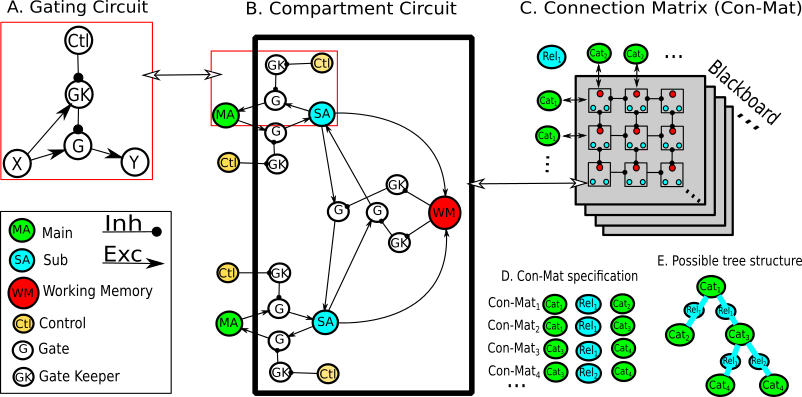
\includegraphics[width=1.00\columnwidth]{figures/gating_circuit3/gating_circuit3}
    \caption{The Neural Blackboard architecture.
      \textbf{A.} Gating circuit that allows the implementation of conditional neural activity transfer between Neural assemblies X and Y through a gate assembly.
      The gate keeper assembly (GK) is activated by the X assembly and then inhibits the gate assembly (G).
      To let information flow through the gate assembly, a control assembly (Ctl) must therefore inhibit the gate keeper assembly.
      \textbf{B.} Architecture of a single compartment circuit of a connection matrix.
      Six gating circuits are arranged in a way that makes conditional bidirectional neural activity flow between two main assemblies possible.
      Control assemblies regulate the direction of information flow and allow the activation of sub assemblies.
      The two sub assemblies excite the working memory assembly which, once activated, encode the binding of the main assemblies and allow activation to flow between them if the controls allow it too.
      \textbf{C.} Each connection matrix contain n by m compartment circuits that encode the same relationship type between the same pair of assembly categories.
      There are $m$ available assemblies for one category and $n$ available assemblies for the complementary category and only one cell circuit can activate its working memory assembly to link two particular assemblies due to mutual row and column inhibition of cells in the connection matrix.
      The size of the connection matrix effectively represents memory limitations.
      A blackboard is composed of an arbitrary number of connection matrices that encode different relationship types for a pair of assembly categories.
      \textbf{D.} A blackboard is composed of multiple connection matrices, where each of them is defined by two node categories and a relationship type between them.
      \textbf{E.} Example of a possible tree structure that can be represented based on the specified connection matrices. }
      \label{Blackboard}
  \end{center}
\end{figure}


Nodes in Figures {\ref{Blackboard}}.A and {\ref{Blackboard}}.B represent neural assemblies that can be interpreted as linked spiking neural populations.
The most basic component of the NBA is a ``Gating Circuit'' illustrated in Figure {\ref{Blackboard}}.A.
The main idea is that neural activity would flow from the assembly X to the assembly Y, but is blockedby the Gake Keeper (GK) assembly, 
which itself is excited by assembly X.
So to allow directional activity flow from X to Y, a Control (Ctl) assembly has to inhibit the GK assembly.
Notice that it is trivial to extend the gating circuit for bidirectional control of activity flow as illustrated in Figure {\ref{Blackboard}}.B.
Introducing bidirectional conditional control signals is what gives the NBA the possibility of implementing separately queries like 'what follows X?' or 'what follows Y?'.

The second basic component of the NBA is a proposal for working memory (WM).
Persistent neural activity in response to stimuli is considered to be the neural process underlying active (working) memory, and its implementation is hypothesized to be based on excitatory reverberation\cite{wang2001synaptic}.
Based on this, the NBA considers a Delay Activity\cite{de_Kamps_2005} mechanism as a biologically plausible implementation of WM. \notenewMdK{Consider Brunel and Wang.}.
\notenewMP{is this mini intro fine?}.
It consists on a neural assembly, that after being excited beyond a certain threshold, achieved by the coactivation of input populations, will maintain a constant amount of activation for a short period of time. By maintaining its activity, WM acts as a short lived bidirectional link between two assemblies. This mechanism can be considered as the creation of an implicit pointer from one assembly to the other, such that future reactivation of one assembly can be driven from the other to perform query operations. This conforms a ``Memory Circuit'' as depicted in Figure {\ref{Blackboard}}.B.

Two bidirectional ``Gating Circuits'' connected by a ``Memory Circuit'' form a ``Compartment Circuit'' capable of implementing variable binding and query operations.
The key point of this circuit is that Main assemblies (MA), representing grounded concepts or instances of variables types, activate Sub assemblies (SA) 
if a control signal driven by another mechanism allows it.
Then coactivation of SAs is what realizes a temporary binding of MAs by activating WM.
So one ``Compartment Circuit'' models specifically the neural activity of a variable binding operation.
It is operated by a mechanism that drives control signals simultaneously in multiple ``Compartment Circuits'' to instantiate binary tree like data structures on which query/unbinding operations can be performed later. 

As might be evident by now, applying the NBA to syntactic processing in language consists of two simple assumptions.
First, equating the parsing mechanism to the control mechanism that coordinate binding events of words and word types and phrase types.
Second, determining the number of compartment circuits necessary to instantiate a complete syntactic structure and the content of MA nodes from a grammar theory.
In this work we will only employ a phrase grammar and bottom-up parsing scheme following theoretical assumptions of selected neuroimaging experiments.
Nonetheless, a promising feature of the NBA is that it has the flexibility to test any arbitrary parsing mechanism incorporating top-down considerations and an important variety of alternative theories of grammar based on binary trees.
For example dependency grammars that assume multiple direct word bindings instead of the hierarchical phrase bindings modelled in this work have been employed in previous simulations\cite{van_der_Velde_2010}.

To understand how a sentence is processed in the NBA, let us consider first the simplest case of binding two words, like ``Sad student'', 
belonging to grammatical categories instantiated in the MAs of one ``Compartment Circuit'', such that one MA is an ``Adjective'' corresponding to ``sad'' and the other one 
is a ``Noun'' corresponding to ``student''.
The MAs activate with timings corresponding to word presentation, so we are assuming that words were recognized to motivate their corresponding instantiated grammatical 
categories before we attempt to link them.
Then an assumed parsing mechanism determines that a link operating on ``Adjective'' and ``Noun'' types is necessary in the blackboard, driving activity in several 
``Compartment Circuits'' from which only one, that we consider as the recruited ``Comparment Circuit'', completes coactivation of SAs to drive WM and realize binding between the word types.

In the case of a complete phrase, like ``Fat sad student'', if we are assuming the instantiation of phrase types that form a hierarchical tree theorized by a phrase grammar, 
then the time at which the binding of the instantiated grammatical categories of ``sad student'' takes place would be the time at which a ``Noun Phrase'' is activated and bound 
to the ``Adjective'' corresponding to ``Ten''.

Finally, a ``Connection Matrix'', portrayed in Figure {\ref{Blackboard}}.C, allows the implementation of a complete ``Blackboard''.
It contains variable type relations learned by the ``Blackboard'' as sets of mutually inhibitory ``Compartment Circuits'' that enable the selection of the 
``Compartment Circuits'' requested by the control mechanism.
We portray the ``Blackboard'' as a regular grid for illustrative purposes, although there is already a proof of concept implementation with 
randomly connected networks\cite{van_der_Velde_2011}.
Also implementing a general syntactic control mechanism should be feasible. As suggested by the Feed-forward artificial 
neural networks employed in previous NBA simulations~\cite{van_der_Velde_2010} and recent state of the art feedforward network architectures that have shown top performance for diverse language parsing tasks~\cite{andor2016globally}.
Moreover a more recent proposed extension of the NBA, that imitates the motor circuit of the marine mollusk Tritonia diomedea, 
shows how to generate patterns for sequential activation control\cite{van_Dijk_2015}.
Simulating these higher level mechanisms is a task out of the scope of this work, since we focus specifically on reproducing the neural signatures of variable binding operations.


\section{Methods}

{\label{488128}}

\subsection{Simulation framework}\label{simulation-framework}

We assume that the NBA lives in the cortex, and seek a good compromise between realistic modelling of the cortical dynamics and the tractability of the simulation.
State-of-the-art simulations of larger cortical structures are based on point model neurons that allow the inclusion of biological details such as synaptic dynamics and adaptation, but are restricted to about the size of a cortical column \cite{potjans2012cell}.
For larger scale networks, such as ours, a population-based approach is currently the only feasible approach.
The two choices are: rate based models or population density techniques (PDTs).
In rate based models, the population is described by a single variable, usually related to the population firing rate or average membrane potential of neurons in the population. 
A prominent example is the  Wilson-Cowan equation \cite{wilson1972excitatory}, which describes the dynamics of the population activity as a first order linear differential equation driven by inputs.
Another example is the Jansen-Rit model \cite{jansen1995electroencephalogram}, which is primarily motivated by phenomenological considerations.
In both examples, the relationship with the underlying neural state is unclear. We have opted for PDTs, also a population based approach, but one where the relationship with the dynamics of a group of spiking point model neurons can be made rigorous.
Although they are computationally more expensive than rate based models, they are easier to manage than a full-blown model using spiking neurons, which would need hundreds of thousands of neurons at the scale of the cortical network considered here.
We will briefly set out the assumptions that we use in modelling populations and describe the numerical methods involved.

Consider a leaky-integrate-and-fire (LIF) neuron, which is characterized by a single state variable: the membrane potential.
If the neuron has a potential different from its equilibrium potential, or when it experiences an external drive, for example generated by a synaptic current, the potential evolves according to:

\begin{equation}
\tau \frac{dV}{dt} = -(V - V_{rev}) + I(t).
\label{eq-lif}
\end{equation}

Here $V$ is the membrane potential in V, $\tau$ the membrane time constant in s, $V_{rev}$ the reversal potential and $I(t)$ and external current, which may comprise contributions from other neurons in the form of spikes, and therefore may be stochastic.
If the membrane is driven far above the equilibrium potential, at a potential $V_{th}$, the threshold, the neuron spikes.
We assume it will be inactive for an absolute refractive period $\tau_{ref}$ and then finds itself reset to the equilibrium potential after that.  
This scenario is easy to simulate: using a simulator like NEST \cite{gewaltig2007nest}, or BRIAN \cite{stimberg2014equation}, one can create populations of LIF neurons.
In the simplest case a population is driven by synthetically generated input spike trains, where the spike train events are created by a random generators.
The default assumption is that inter-spike intervals are Poisson distributed, although this can be extended to non-Markov processes \cite{lai2017population}.
It is clear that $I(t)$ in Eq. \ref{eq-lif} now should be considered as a stochastic variable and that the threshold crossings of LIF neurons themselves are stochastic events as a consequence.
Fig. \ref{pdtcase} A  demonstrates a simple scenario: a population of 10000 LIF neurons, driven by a stochastic input - Poisson generated spike trains, where each LIF neuron experiences about 800 input spikes per second.
The simulation shows a spike raster of the population response:
first nothing: although each LIF neuron receives input spikes and as a consequence has its membrane potential driven up, none of the neurons have reached threshold;
then a spike volley: most neurons hit threshold at approximately the same time;
followed by a period of relative silence: only interrupted by a few stragglers;
at last a gradually achieved final neural state of asynchronous random firing.
More complex networks can be formed by feeding the output spikes of one population into other populations.

This is a fascinating but unwieldy process and statistical methods have been used to describe it at the population level \cite{stein1967some,knight1972dynamics,omurtag2000simulation}.
A population is described by a density function, which expresses how the population is distributed over state space.
For LIF neurons this is a function $\rho(V)$, where $\rho(V)dV$ is the fraction of neurons with their membrane potential in interval $[V, V + dV)$ (when we integrate the density function over a certain state interval, we will refer to the  result as  the amount of \emph{mass} in that interval).
The initial distribution of the neurons in the population must be chosen, but the evolution of the density is tractable.
It is clear that neurons move through state space due to the deterministic neural dynamics, Eq \ref{eq-lif} for LIF neurons, and also go transitions due to the input spikes.
The collective contribution of the stochastic process to the evolution of the density profile can be  modelled using a Poisson master equation \cite{crispin1994handbook}; the contribution of the deterministic dynamics  can be modelled using an advection equation (see \cite{omurtag2000simulation} for a lucid explanation). 


As a consequence, the process of simulating thousands of neurons is now replaced by modelling the evolution of a density which is given by a single equation:

\begin{equation}
\frac{\partial \rho}{\partial t} -\frac{1}{\tau}\frac{\partial}{\partial v}(\rho v) = \int dh p(h) \nu (\rho(v - h) -\rho(v)),
\label{eq-synapse}
\end{equation} 

Here $p(h)$ is the distribution of synaptic efficacies, $\nu$ the frequency of the incoming spike trains, $\rho$ the density function, $t$ the time since start of simulation and $v$ the membrane potential.
Mass that is being pushed across threshold corresponds to neurons spiking; consequently  the firing rate of the population can be calculated directly from the mass flux across threshold.

Efficient and stable simulation methods are available \cite{nykamp2000population, de2003simple, de2013generic, iyer2013influence}, and remarkably, the process of solving Eq. \ref{eq-synapse} is computationally less expensive for LIF neurons than the direct simulation using NEST \cite{nykamp2000population}.
The process of keeping track of a single density function, and the communication between populations using firing rates rather than individual spikes, frees the modeller from keeping track of thousands of spikes per second and leads to simpler simulations.
Figure \ref{pdtcase} shows the very close correspondence between direct simulations of LIF spiking neurons and population density results.
It shows, first, that the simulation results indeed are very close to that of the spiking simulation, and second, that Wilson-Cowan dynamics must be tuned in a way that PDTs do not: the correct steady state activation must be provided to the Wilson-Cowan dynamics in the form of a sigmoid, while in PDTs the correct steady state firing rate is calculated from first principles - input firing rate, synaptic efficacies and neural parameters - without any need for tuning. 


\begin{figure}[h!]
  \begin{center}
    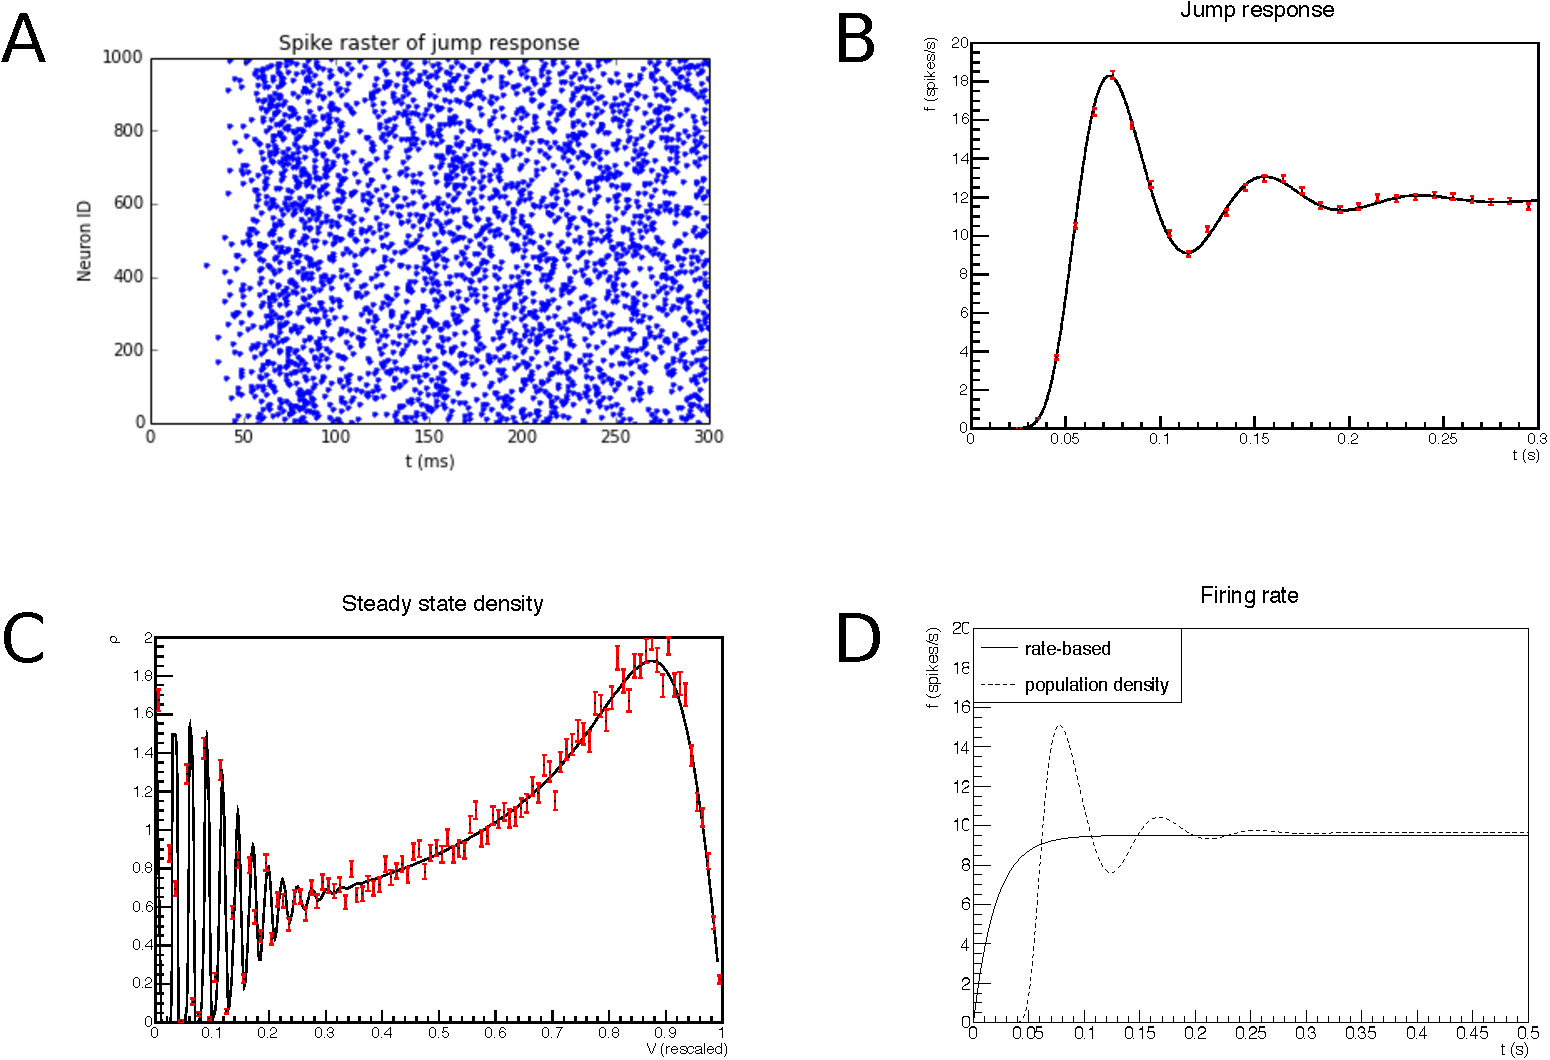
\includegraphics[width=1.0\columnwidth]{figures/pdt_overview.pdf}

    \caption{\textbf{A.} A spike raster showing an LIF population undergoing a jump response.
        Neurons are at equilbrium at $t = 0$. From $t=0$ each neuron receives a Poisson distributed input spike train ($\lambda$ = 800 Hz, $h= 0.03$, i.e. an input spike raises the PSP by 3\% of the difference between threshold and equilibrium potential, $\tau = 50$ ms, following \cite{omurtag2000simulation}).
        \textbf{B.} Firing rate calculated from the PDT method (solid curve), compared to firing rate from spiking neuron simulation (red markers).
        \textbf{C.} The density calculated by the PDT method (solid curve) at $t=0.3$ s, compared to a histogram of the membrane potential over the population at the
        same time.
        \textbf{D.} Wilson-Cowan prediction for the firing rate, compared to PDT result. Importantly, Wilson-Cowan output must be tuned: the steady state value to which it converges is not predicted by the Wilson-Cowan equations, but must be provided as a sigmoid. 
       In contrast, the PDT method calculates the firing rate from first priciples, and agrees well with the spiking neuron simulation, within statistics.
      }
\label{pdt_case}
  \end{center}
\end{figure}


The population density formalism can be extended to higher dimensional models.
For example, the adaptive-exponential-integrate-and-fire neuron (AdEx) \cite{brette2005adaptive} is a two dimensional model that has the membrane potential and an adaptivity parameter as a variable.
Consequently, the state space is two dimensional.
The motivation behind this model is that first, it includes adaptation, and second that it is the effective approximation of the complex conductance-based processes that take place in a real neuron.
The equations of the model are:

We consider the AdEx model as presented by Brette and Gerstner \cite{brette2005adaptive}, which describes individual neurons by the following equations:
\begin{align}
  C_m \frac{dV}{dt}    & =  -g_l(V - E_l)  + g_l e^{ \frac{(V - V_T)}{\Delta_{T}}} \\
  \tau_w \frac{dw}{dt} & =  a(V-E_l) -w \nonumber
\end{align}

Where $C_m$ is the membrane capacitance, $g_l$ the leak conductance, $E_l$ the leak potential (equivalent to the reversal potential for the LIF), $V_T$ a threshold potential, $\Delta_T$ a shape parameter for the spike, $\tau_w$ the adaptation time constant, $a$ the subthreshold adaptation parameter,  $V$ the membrane potential and $w$ the adaptation parameter. Upon a spike, the neuron is undergoes a transition in $w$: $w \rightarrow w +b$, where $b$ is the spike adaptation parameter.
We use the parameters given by Brette and Gerstner (2005).


\begin{figure}[h!]
  \begin{center}
    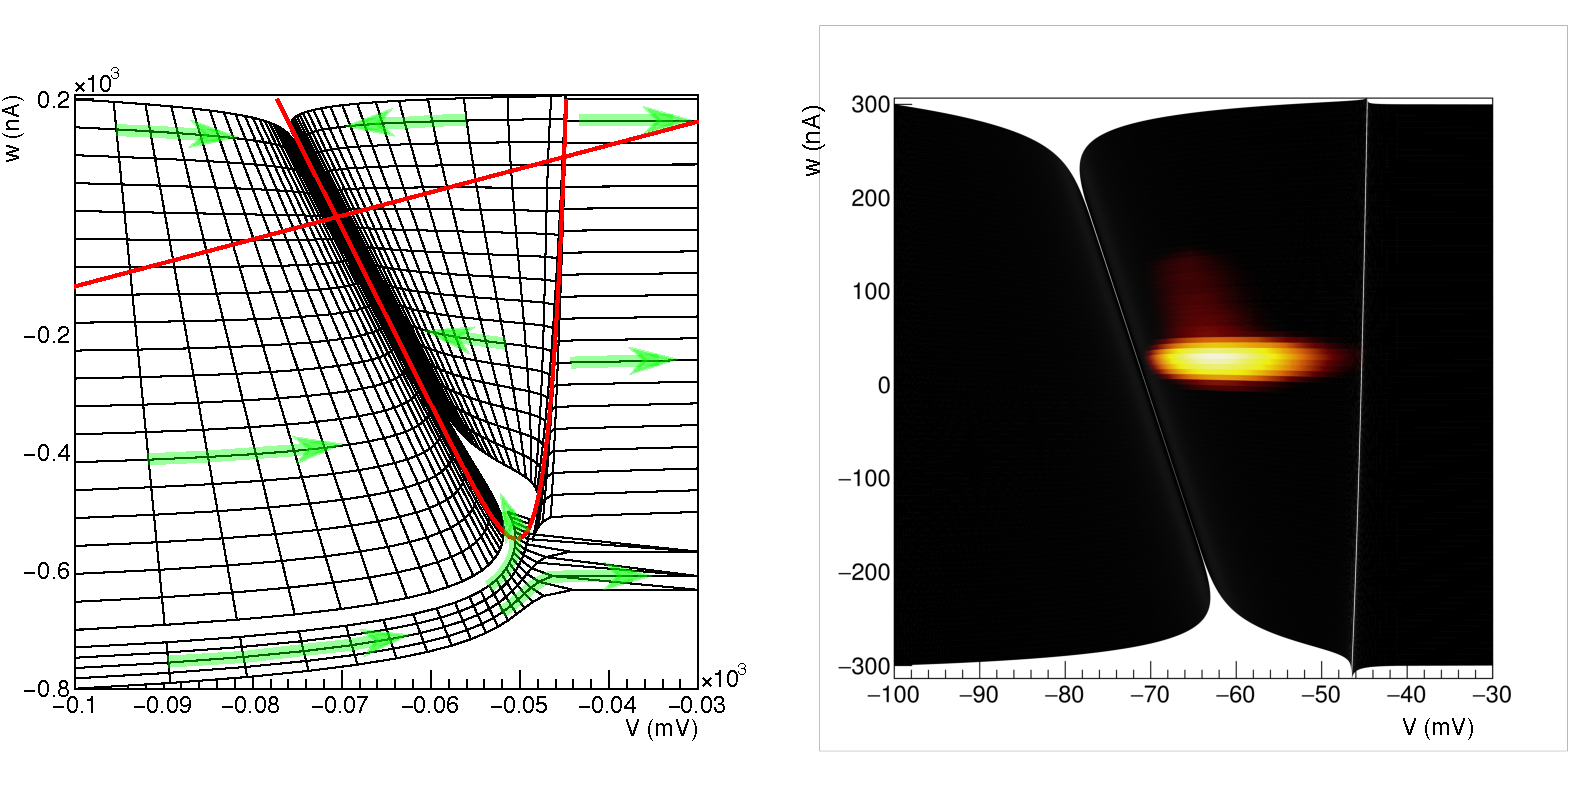
\includegraphics[width=1.0\columnwidth]{figures/aexp_overview.pdf}
    \caption{{AdEx dynamics {\label{fig-adex}} Left: Overview of AdEx dynamics.
        Right: a heat plot of the density profile during simulation. On the horizontal axis the membrane potential, on the vertical axis the adaptivity parameter. Note that
 the right figure constitutes a considerable reduction of state space compared to left. For the connectivity parameters we use, the state space on the right is the
part of state space reachable by dynamics.
      }}
  \end{center}
\end{figure}

We illustrate the dynamics of the neuron in Fig. \ref{fig-adex}.
The direction of the dynamics is shown by arrows, the speed of the dynamics by the size of the cells:
big cells implies fast dynamics as the cells represent equidistant time steps.
This shows that at $w =0$ dynamics are leaky,  i.e. towards the equilibrium, except at high values of $V$, on the right, which corresponds to spike generation.
At high values of $w$, there are two effects: stronger leak (larger cells) and a lower (more negative) equilibrium potential, which makes it harder for a cell at high $w$ to be driven across threshold, precisely the effect one expects due to adaptation.
At low $w$, the opposite happens: cells become more excitable.
For very low $w$ values, which can not be reached under cortical conditions, at least not for the parameters we used, there is the theoretical probability of a rebound (neuron always spikes).

A density function now lives in this two dimensional space: $\rho(V,w)$.
The evolution equation is a direct generalization of Eq. \ref{eq-synapse}.
For a model with $n$ state variables $\vec{V}$, a point model takes the form:
\begin{equation}
\tau \frac{d \vec{V}}{dt} = \vec{F}(\vec{V})
\end{equation}
and the density equation:
\begin{equation}
\frac{\partial \rho}{\partial t} + \frac{\partial}{\partial \vec{V}} \cdot \frac{( \vec{F} \rho)}{\tau} = \int dh p(h) \nu (\rho(\vec{V} - \vec{h}) -\rho(\vec{V}))
\end{equation},
where $\vec{h}$ represents the effect of an input spike.

We represent the density function by a heat plot on state space: the highest values or white, low values are red.
We are able to simulate the density function by a method analogous to that of \cite{de2013generica,iyer2013influence}, generalized to two dimensions.
In Fig. \ref{fig-adex} we show the result of a simulation: the density function as a fixed point in time.
As before, we can calculate the firing rate of the population by calculating the the flux across threshold (which is still given by $V= V_{threshold}$, i.e. the right hand side of the grid).

The simulation software, MIIND, is publicly available \url{http://miind.sf.net}. The LIF version of the algorithm has been available for some time \cite{de_Kamps_2008}, while 
the two dimensional version has become available recently \cite{dekamps2017b}.


\subsection{NBA simulation}\label{architectural-decisions}

Previous simulations of the NBA approximate the mean activity of neural assemblies with Wilson Cowan dynamics \cite{Frank_2014}.
Nonetheless, as explained in section \ref{simulation-framework}, direct simulations of leaky-integrate-and-fire (LIF) neurons \cite{omurtag2000simulation} have different transient behaviour than the dynamics described by the Wilson Cowan equations.Since we are interested in modelling the transient dynamics of variable binding in order to compare 
the simulation with real temporally detailed patterns of intracortical neural measurements like ECoG, we feel the need to model spiking neuron dynamics is important.

The decision to use AdEx, rather than LIF neurons has two motivations: first, adaptation is ubiquitous and its inclusion has a substantial impact on the dynamical range
allowed within the constraints of the blackboard architecture. Second,  it has been shown that 2D models, like AdEx, can already predict correctly 96\% of the spikes of 
detailed conductance models\cite{brette2005adaptive}.  Also, this model reproduces many known electrophysiological features, as can be appreciated in the spike-frequency adaptation review of Benda et al. \cite{Benda_2003,Benda_2014}. Our approach is consistent with a trend towards simpler, geometrically motivated  2D   models  that preserve the essence of more complex biophysically motivated models \cite{izhikevich}.


AdEx is now available in  MIIND. Although it is two orders of magnitude more computationally expensive than a LIF model, it is still feasible to implement 
it in a circuit with only tens of populations like the one we will simulate.
\noteMdK{What does that mean?}
To our knowledge this is the first time that the AdEx model will be employed to approximate the neural dynamics of a circuit of this magnitude reproducing cognitive function.

In the case of Delay Activity (DA) populations like Working Memory (WM), we decided as a first approach to model such a mechanism artificially.
We plan to address the different alternatives to model persistent cortical activity with interacting neural populations in future work.
As suggested by de Kamps\cite{de_Kamps_2005} not only models of recurrent excitation but also recurrent inhibition can account for this phenomena.
In the current simulation, a constant firing rate for DAs is kicked off by a specified level of input, resulting in activation  that is sustained for a predetermined period of time.
Contrary to previous simulations \cite{velde2015ambiguity}, we do not consider Sub-Assemblies (SAs) as DA populations.
We find that SAs can show rich and interesting dynamics just by fulfilling their function of mediating activation for WM.

We model Main-Assemblies (MAs)  as receiving input from DA populations, representing word types in some cases, and WM populations representing phrase types in other cases.
We do this to satisfy the assumptions of a phrase grammar that requires representation of deep tree hierarchical structures, so that we can separate the notion of a phrase resulting from previous word type bindings stored in WM, from the recruitment of MAs representing word grammatical category instantiations that take place during sentence processing.
Note that for other grammar types, like dependency grammars considered in previous NBA simulations\cite{velde2015ambiguity}, to consider words as nodes in their syntactic representations, we would only need to model word types for the MAs of the necessary compartment circuits.


\subsection{Compartment circuit parameters}\label{compartment-circuit-parameters}

The compartment circuit contains two different types of neural populations.
Artificial neural populations following a boxcar event model, shown in Figure \ref{circuit_spec}.B and biological neural populations following LIF or AdEx neural models.
%Both biological neural models have a wide range of parameters that have been tuned in the literature to follow the behavior of a regular spiking pyramidal cell in the 
%cortex according to electro-physiological measurements.
\noteMdK{I think you've said this before, I commented it out.}
We took LIF parameters from Omurtag et al. (2000) \cite{omurtag2000simulation} and AdEx parameters
from Brette and Gertsner \cite{Brette_2005}.

\begin{figure}[h!]
  \begin{center}
    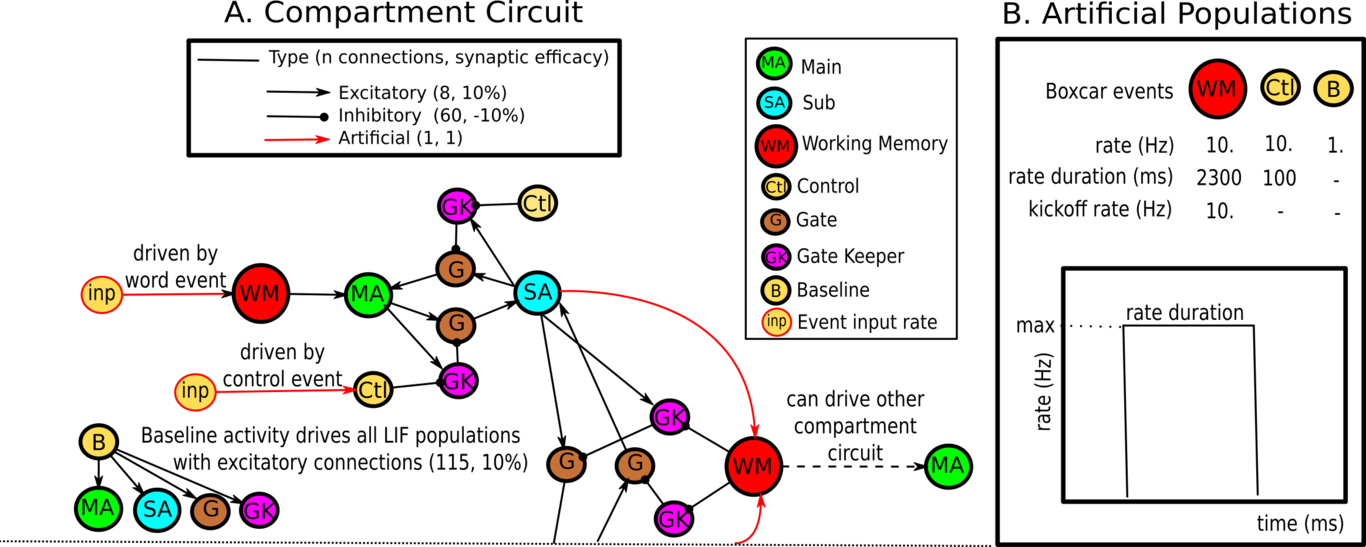
\includegraphics[width=1.00\columnwidth]{figures/circuit_specs3/circuit_specs3}
    \caption{{Compartment circuit example {\label{circuit_spec}} A.
Details
        of the Compartment Circuit implementation.
Only half of the
        circuit is shown since the design is symmetric.
The baseline
        (B) and Event input (Inp) populations are part of the
        simulation and not of the original abstract circuit proposal.
        B.
The behavior of the artificial neural populations and their
        selected parameters is shown%
      }}
  \end{center}
\end{figure}

As a first step we wanted to only explore the general behavior of the circuit of neural populations following well studied sets of parameters.
Nonetheless it is clear that studying the neural dynamics of specific brain regions might require adapting the parameters of the neural models to local measurements.
\noteMdK{Is the below relevant?}
It could also be important to consider parallely multiple neuron typologies and modelling their corresponding microcircuitry of cortical columns, as attempted already with LIF models, to simulate local field potentials for a very small patch of cortex\cite{Mazzoni_2015,Hagen_2015}.

Each neural population is either excitatory or inhibitory; a population that is excitatory (inhibitory) on one population is excitatory (inhibitory) on others as well, respecting Dale's law. The dynamics of most populations is given by the PDTs and ultimately determined by the underlying model of spiking neurons, but there are a few populations where
we make simplications:  The biophysical mechanisms of WM
are still not understood completely, but the existence of delay activity as phenomenon is relatively uncontroversial, so we model working memory by assuming that after stimulation it retains its activation abover a certain threshold for a given period of time, after the stimulus causing it has been removed..


\noteMdK{What does conformed mean here? Comprised?}
The biological neural populations are conformed by a pair of Main Assemblies (MA), a pair of Sub Assemblies (SA), six Gate Assemblies (G) and six Gate Keeper Assemblies (GK).
On the other hand the artificial neural populations are conformed by Control assemblies (Ctl), Working memory assemblies (WM), Event Input Assemblies (Inp) and a Baseline Assembly (B) that drives baseline neural activity.
A complete diagram of the compartment circuit with example parameter values for LIF populations is given in Figure \ref{circuit_spec}.

\noteMdK{I think it's confusing to talk about 'biological' and 'artificial' populations. At the end of the day, even the 'artificial' populations model biological events.
What you can say is: there is a group of populations where we have to simplify dynamics: in working memory we assume the existence of delay activity and model this
phenomenologically; we also model external input events as given. But for most population we model the response according to the underlying biophysical neural model.} 


We use a boxcar event model for persistant activity. This model requires specification of the starting point of events, the persistent firing rate of the population and the duration of the persistent activity.
In the case of the delay activity of WM we also have to provide a kickoff input rate threshold that automatically triggers the boxcar event instead of providing a start time point.
The duration of persistent activity was pragmatically set up long enough for the neural dynamics to reach steady state and allowthe formation of  all required bindings between phrase types and 
word types.
Finally the persistent activity rate and kickoff rate threshold were arbitrarily selected from possible parameter range values as a result of simulations of the circuit dynamics that will become clear in the following section.

Selecting firing rates to tune the compartment circuit is a complex task given the contrast between the extremely simplified circuit and real neural networks that contain multiple types of neurons with diverging behavior across cortical layers \cite{Wohrer_2013}.
Wohrer et al \cite{Wohrer_2013} show, from measurements in rat cortex, that the actual firing rate distributions of neural networks do not differ much between resting state and evoked activity.
The small difference would come from very few neurons that manage to drive up the mean firing rate in recordings while most neurons in the population are almost silent, some with rates as low as 0.1 Hz \cite{Kerr_2005}, whose activity might not even be picked up by most recording devices.
Although theoretical analysis of the distribution of firing rates in randomly recurrently connected networks of LIF neurons near the fluctuation-driven regime suggests considering mean firing rates around 6.4 Hz \cite{Roxin_2011}.
Based on the review of Wohrer et al. \cite{Wohrer_2013}, particularly on the firing rate in motor areas of behaving macaques, we decided to kickstart biological neural populations activity up to a conservative baseline firing rate of 1 Hz and study the neural dynamics of circuit input firing rates of up to 10Hz.

There are two parameters governing transmission of neural activity between neural populations.
First, the synaptic efficacy of connections, which was setup to be uniform across the circuit under the lack of appropriate hypothesis to tinker it in a detailed manner.
\noteMdK{The next sentence is incomprehensible.}
According to London \cite{London_2002}, current understanding of synapsis is limited and even contextual measurements of efficacy might be more appropriate to understand the impact of synaptic input on spike output that actual set parameters of the synapse.
Moreover recent evidence \cite{Briggs_2013} shows that synaptic efficacy might be modulated by attention processes and is naive to consider it as a fixed parameter in a circuit.
The study of Briggs \cite{Briggs_2013} suggest that synchronous firing of neurons with the same input has probabilities between 3.1 and 7.6 while single firing has probabilities ranging from 28\% to 36\% depending on the type of neurons considered and the attention state.
Accordingly, we decided to verify, through simulations of a  sub-circuit, the effect that synaptic efficacy has on the circuit temporal dynamics, contrasting a low (10\%) and high (30\%), where percentages are taken with respect to the difference between equilibrium and threshold potential value of synaptic efficacy for both LIF and AdEx populations.

\noteMdK{You suddely start disuccing results of simulations here, of experiments that you will be performing later. Highly confusing. Consider moving to the next section.}

This allowed us to verify if the tradeoff between efficacy and number of connections was a trivial one, simply requiring more connections when assuming a lower efficacy to attain similar ouput firing rates for the same input rates, which, as will be show in the results section, was not the case for AdEx populations.
Nonetheless the difference in the qualitative nature of the temporal dynamics was confirmed to not be crucial for the circuit setup, so for the remaining simulations we employed the more conservative 10\% synaptic efficacy regime.

The second parameter governing transmission of neural activity was the number of connections between a pair of neural populations.
Unlike synaptic efficacy, the number of connections were determined from a series of simulation experiments.
First the number of connections from baseline persistent activity was set such that, during rest, the circuit steady state activity would stabilize around 1 Hz.
The number of baseline connections necessary is a function of input firing rate, synaptic efficacy and neural model, such that a lower synaptic efficacy required a higher number of connections.
Then the number of connections coming from excitatory populations was determined such that bidirectional gating circuits would have a stable steady state firing rate when both Gs allow neural activity to be transmitted.
Finally the number of connections coming from inhibitory nodes were setup high enough to block neural activity flow in a gating circuit, which means that GKs driven by MAs would be able to completely inhibit activity in Gs.
Our simple approach to neural rate transmission ignores many intricacies like activity regimes that might allow rich internal computations.
\cite{Ostojic_2014}.
Also connections distribution might have an impact in spike based communication \cite{Teramae_2012}.
Still we decided to keep connections between populations as simple and homogeneous as possible for a first approach.

\subsection{Simulation experiments performed}\label{simulation-experiments-performed}

Since it is possible to tune the circuit to reproduce a wide range of firing rate absolute values under which circuit dynamics are similar and stable, we simply aimed at picking reasonable parameter values such that the circuit would maintain overall modest firing rate values with respect to the literature of neural measurements.
To setup parameters and compare in detail the compartment circuit dynamics for LIF and AdEx neural populations, four simulation experiments were performed taking different sub-circuits into account.
A diagram of each sub-circuit is shown in Figure \ref{sub_circuits}.

\begin{figure}[h!]
  \begin{center}
    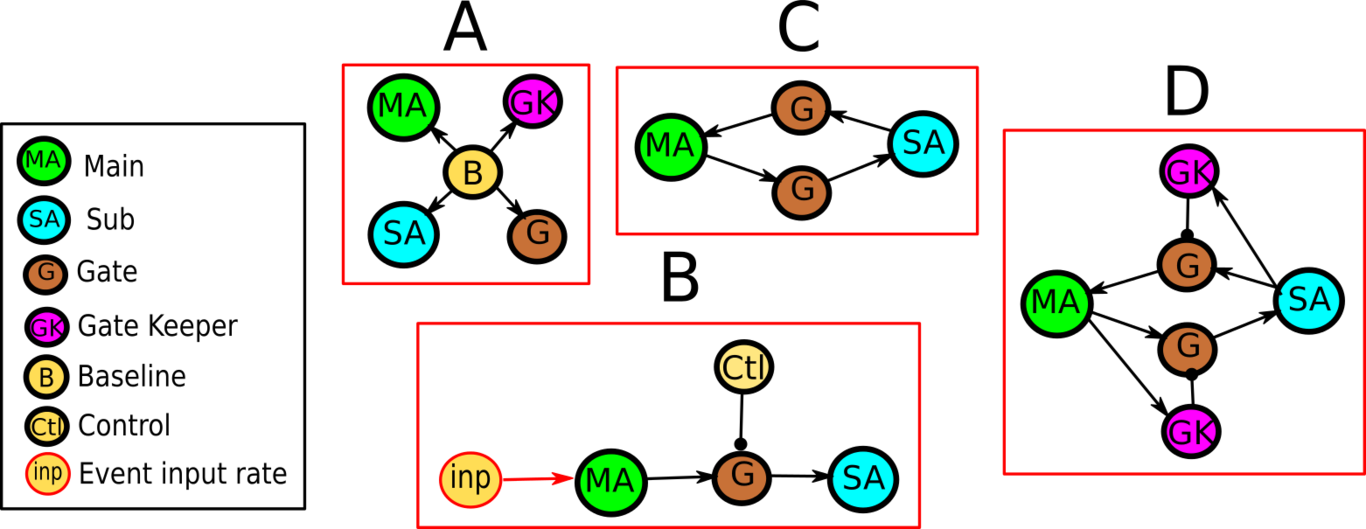
\includegraphics[width=0.70\columnwidth]{figures/sub_circuits3/sub_circuits3}
    \caption{Sub-circuit simulation topologies.
      Each number corresponds to its respective experiment.
      For better visualization all baseline nodes are excluded from the topologies.
      A. Single neural population driven by baseline activity.
      This topology~ reminds of the fact that all MA, SA, G and GK populations are driven initially in the same way by a persistent baseline fixed rate.
      B. Chain of populations where activity is temporally interrupted by a control node.
      C. Closed loop formed by MA, SA and Gs.
      D. Closed loop broken by the addition of GKs. {\label{sub_circuits}}%
    }
  \end{center}
\end{figure}

The first simulation simply consists of the activity of one neural population driven by a fixed activity rate of 1 Hz.
We used this simulation to explore the necessary number of baseline connections to drive baseline activity in the circuit to approximately 1 Hz.
The second simulation allowed us to explore how neural activity flows through a chain of neural populations being regulated by a control mechanism.
The third simulation explores how neural activity is enhanced by a closed loop between a MA and SA, since it will be the case in the memory sub-circuit that activity is allowed to flow bidirectionally once the WM delay activity is unleashed.
Finally the fourth simulation consists on adding GKs to the closed loop sub-circuit of the second simulation to explore how many inhibitory connections are necessary to keep activity from flowing in the circuit unless the control mechanism allows it.

After determining reasonable parameter values, we simulated the complete circuit, shown in Figure \ref{circuit_spec}, for both LIF and AdEX neural populations.
Then we compared the resulting neural patterns of the MA, SA, G and GK neural populations to binding and constituency effects available in the neuroimaging literature.

We simulate the binding activity related to the processing of complete phrases, by assuming a syntactic tree structure given by a phrase grammar theory and the order of control events given by a bottom up parsing scheme.
\noteMdK{What does parallely refer to in the next sentence?}
As a first simplified approximation to the NBA dynamics, we instantiated parallely only the required compartment circuits to represent the complete assumed tree structure.
We obtain the entire phrase neural time series, by summing activity across similar node categories of the multiple compartment circuits required.

First, we show similarities between the activity of simple phrases and ECoG time series patterns of binding revealed by Nelson et al\cite{Nelson_2017}.
\noteMdK{Where do you do this comparison? Here? Later?}
We naively compare the firing rates of our simulation directly to the patterns observed in ECoG recordings, considering the correlation that exist between the high gamma power of local field potential signals and firing rates\cite{Ray_2011,Manning_2009}.
Nonetheless a quantitative comparison would require a more careful consideration, employing recent models tuned to electro-physiological measurements that offer a way to translate neural activity to local field potentials\cite{Mazzoni_2015,Hagen_2015}.

Second, we concatenate simple phrases to reproduce the stimuli of Pallier \emph{et al.} (2011)\cite{Pallier_2011}.
Then we convolve the stimuli neural time series with the Glover Hemodynamic Response Function\cite{Glover_1999}.
This allowed us to approximate the hemodynamic constituency effects depicted by Pallier et al. (2011)\cite{Pallier_2011}.
We show that the sublinear function given by the number of constituents, governing the amplitude of HRF responses for the different stimuli categories, is naturally approximated by the binding events assumed by the NBA, alongside an increasing pattern in HRF peak onsets.

Since the quantitative level of neural activity can be easily tuned for a wide range of parameter values with similar behavior, when comparing the circuit neural dynamics with the neuroimaging literature, we only focused on the qualitative neural temporal patterns observed.
All the C++ scripts behind the circuit and sub-circuit simulations, taking advantage of the MIIND software\cite{de_Kamps_2008}, are accessible in the Blackboard application folder of the MIIND github repository at https://github.com/dekamps/miind.


\section{Results}

{\label{765620}}

\subsection{Sub-circuit simulations}

{\label{152250}}

\subsubsection{Experiment 1: Simple neural population}

{\label{461536}}

The first experiment allowed us to explore the basic temporal behavior of the different neural models under different synaptic efficacy regimes.
It also allowed us to select an appropriate number of baseline connections to tune the steady state firing rate of all LIF and AdEx neural populations to approximately 1Hz while being driven by a persistent artificial 1Hz baseline rate.
As indicated in the topology A of Figure 4, all neural populations are driven identically by a baseline node, so simulating one allow us to get an idea of the behavior of all biological populations in isolation from the circuit connections.

As depicted in Figure 5, the steady state firing rate of LIF populations is a monotonous increasing function of number of connections for both synaptic efficacy values.
We can see from the detailed temporal activity that the firing rate increases gracefully until achieving the steady state after approximately 200ms.
On the other hand, the AdEx populations behavior is qualitatively affected by the synaptic efficacy value chosen.
For a 10\% efficacy the steady state behaves like a monotonous increasing function as in the case of LIF populations but for a 30\% efficacy we observe a concave behavior due to extreme adaptation that limits the steady state rate to a maximum below 1Hz.
If we look at the temporal details, the Adex populations also behave differently from LIF populations.
They portray a sudden increase of activity on initial stimulation that is then driven down by adaptation, achieving a steady state after approximately 600ms.

Based on these observations we decided to consider only the low efficacy regime of 10\% for the remaining simulations.
In the case of LIF populations the higher efficacy would not bring any qualitative modification to the dynamics of the circuit.
In the case of the AdEx population the only important qualitative difference would be constraining the use of the steady state rate of activity, which would itself force a tighter coordination of events.
This more strict event coordination can also be understood from the more permissive low efficacy regime as will become clear in the following simulations and discussion.
Finally we learned that the number of baseline connections that best approximate a 1Hz steady state firing rate are 115 and 1646, for LIF and AdEx populations respectively, which will be fixed for all remaining simulations.

\begin{figure}[h!]
  \begin{center}
    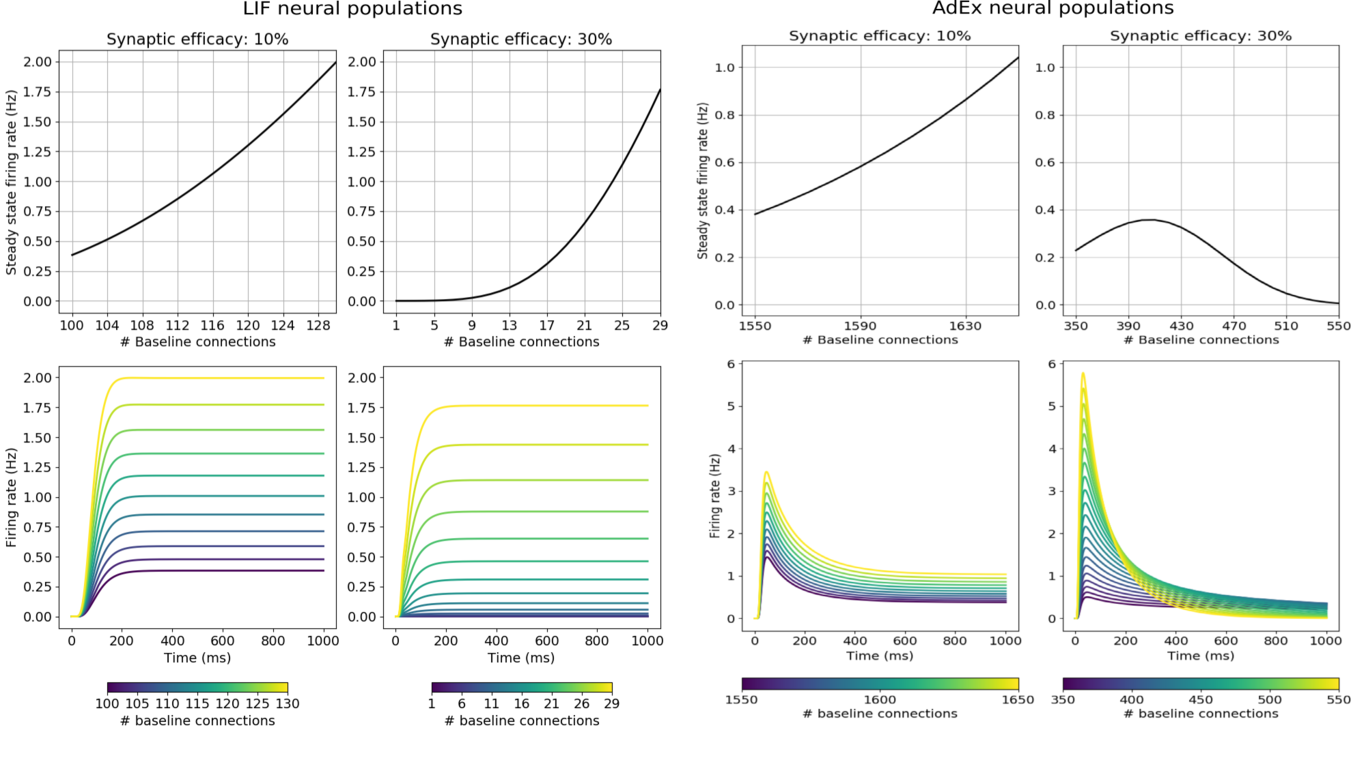
\includegraphics[width=1.00\columnwidth]{figures/experiment_001/experiment_001}
    \caption{Baseline neural dynamics.
      The plots at the top depict how the steady state rate of a neural population relates to the number of baseline connections under a baseline input of 1Hz.
      The plots at the bottom show example temporal dynamics corresponding to its upper plot.}
    \label{674368}

  \end{center}
\end{figure}

\subsubsection{Experiment 2: Neural activity flow and control
  release}\label{experiment-2-neural-activity-flow-and-control-release}

In the second experiment we explored how the coordination of input and control events would affect the rate of activity across a chain of neural populations.
We employed the topology B of Figure 4, in which a fix input rate drives the activity of the sub-circuit during a given time window and is mediated by a control operating under another time window.
This corresponds to a MA that attempts to drive up the activity of G and SA, while a Ctl node inhibits the activity in G and isolates SA activity from the input stimulation.
The input and control events can start at any arbitrary moment for any duration and what interests us are the dynamics of the circuit when inhibition, assumed in the complete circuit to be always present, stops allowing MA to freely excite G and SA.
There are three extreme cases that characterize the circuit behavior.
When the input starts and the circuit achieves the steady state before G inhibition stops (Input first), when G inhibition stops and the circuit achieves a steady state before the input starts (Control first) and when both input starts and inhibition stops at the same moment (Coordinated).
Analyzing this sub-circuit let us determine what kind of input rates are necessary to drive the maximum and steady state rate of SA to some desired activation threshold for WM.
Moreover it gave insight into what are the most constrained type of events for each neural model.

In Figure 6 we portray the neural dynamics of the last population of the chain (SA).
The steady state in a LIF model is achieved at a similar time (under 200 ms) for all event cases.
The Input first and Coordinated events have a similar quantitative behavior, which means that the dynamics of stopping inhibition are insensitive to MA having achieved a steady state from the input stimulation.
Nonetheless starting the input on the absence of inhibition permits higher initial fluctuations of the firing rate and so higher maximum rates of activity.
On the other hand, the AdEx model shows a more complicated behavior.
Due to adaptation effects, the maximum output rate response will depend on the current state of the population.
Basically~the closer the population is to its steady state, the less responsive it will be due to the accumulated adaptation.
In AdEx populations the steady state takes longer to be achieved (just approximated after 400ms) and its convergence rate depends on the input rate and events combination.
Also the maximum firing rate of the dynamics strongly depends on the event case.
Contrary to the LIF model, stopping inhibition in advance minimizes the rate dynamics due to the stronger adaptation present at the steady state of G.
Then starting the input before stopping inhibition improves the rate dynamics at G and SA, which increase the further MA is from achieving a steady state after the input starts and so are maximized with perfect coordination of input and control.

From these observations we learn that the combination of events that reduce the most the rate dynamics depend strongly on the neural model selected.
Being the Input first or Coordinated cases for the LIF model and the Control first case for the AdEx model.
Moreover, as is apparent in Figure 6, the AdEx model requires a higher input rate to achieve modest increases in the steady state of the output rate, which limits the behavior of a circuit of AdEx populations under constant input rates.

\begin{figure}[h!]
  \begin{center}
    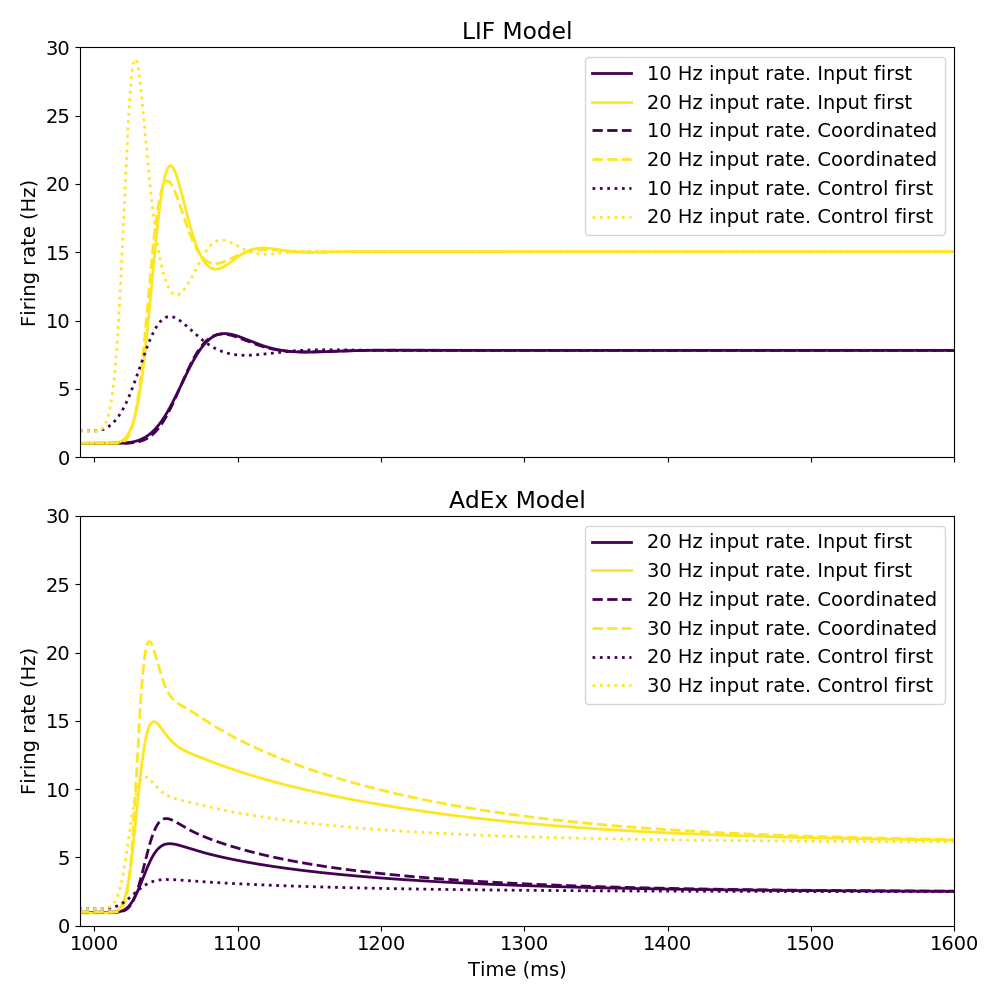
\includegraphics[width=0.70\columnwidth]{figures/experiment2_ctl_plots/experiment2_ctl_plots}

    \caption{Neural dynamics of input and control events.
For each
      neural model two input rates are simulated with the three
      extreme combination of events: Input first, Control first and
      Coordinated.
~9 and 20 excitatory connections are assumed for
      the LIF and AdEx models respectively.
We show the time series of
      the firing rate in the last population of the chain
      (corresponding to a SA node of topology B in Figure 4).
}
    \label{462003}
  \end{center}
\end{figure}

\subsubsection{Experiment 3:~Enhanced neural activity from closed
  loop}

{\label{758539}}

In a third experiment we tested the behavior of the sub-circuit corresponding to topology C of Figure 4.
As was mentioned before there is a number of excitatory connections after which the output rate is higher than the input rate, such that populations wired in a closed loop would enter an uncontrolled self reinforced activity regime.
Since we expect such a loop to exist in our circuit during activation of WM, we had to constraint the number of excitatory connections employed.
Another important implication of the closed loop is that we would expect the steady state activity of the populations to be higher than in their independent states, which also gives a lower bound to the activation threshold that we can select for WM, since otherwise WM would enter a state of perpetual self activation after being activated the first time.
The steady state rate of the closed loop is shown in Figure 7 up to the number of excitatory connections that would lead to an uncontrolled activity regime.

Taking also into consideration the results of the second experiment we can depict valid combinations of input rate, number of excitatory connections and WM activation threshold.
In figure 7 we show the steady state rate (SS) curve for the events combination with the lowest rate dynamics and the maximum rate (Max) curve for the events combination with the highest rate dynamics.
Notice that, as explained in the previous experiment, the relevant combination of events in the analysis are different in the case of LIF and AdEx populations.
These curves delimit four parameter regions with different implications for the behavior of the NBA's memory circuit.
The regions refer to the ranges of values that the WM activation threshold can take according to a given input rate and number of excitatory connections.
The example curves shown in Figure 7 correspond to an input of 10Hz and 25Hz for LIF and AdEx populations respectively.

The perpetual activation region refers to the area below the steady state of the closed loop activity and is independent of input rate.
All other regions depend on the input rate that determines the lowest and highest rate dynamics.
The flexible activation region refers to the area between the closed loop curve and the steady state of the event combination with the lowest rate dynamics.
An activation threshold in that region would secure activation of WM to any combination of events, which makes it the most desirable range for the activation threshold.
The constrained activation region is bounded by the max temporal rate of the highest rate dynamics and represent the range of values for which the timing of input and control events is constrained.
Finally the impossible activation region is above the highest rate dynamics and represent rate values that can not be reached by the circuit dynamics.

Characterizing the activation threshold regions is important to understand the reliability of the circuit when exposed to noisy input rates, arbitrary coordination of events, control mistakes or anticipatory control signals.
With precise control of input rates and the timing of events corresponding to bottom up parsing, one could simply select an activation threshold just above the minimum rate dynamics to secure activation from the activity of two SAs.
Nonetheless there are other scenarios that we should be able to test with parsing schemes diverging from pure bottom-up parsing, if we interpret prediction as anticipated control activation.
In that case, if prediction fails we would be confronted with a control mistake for which we would not want the circuit to perform a binding.
This would be illustrated by an input that drives activity in the first MA of a compartment circuit followed by a control event that allows activity to flow from all MAs, while the second MA never receives the input corresponding to the activation of its concept.
In such a case one would need the threshold to be higher than the minimum of the impossible activation region for a given input rate and number of excitatory connections, such that the input of one SA alone could not trigger WM.
This additional constraint can itself push the activation threshold beyond twice the maximum of the flexible activation region, forcing coordination of at least one input and control event, as can be appreciated for AdEx populations in Figure 7.
To allow anticipatory control mistakes for the complete circuit simulation we selected a combination of 10Hz and 20Hz input rates, 8 and 20 excitatory connections and 10Hz and 9Hz activation thresholds for LIF and AdEx populations respectively.

\begin{figure}[h!]
  \begin{center}
    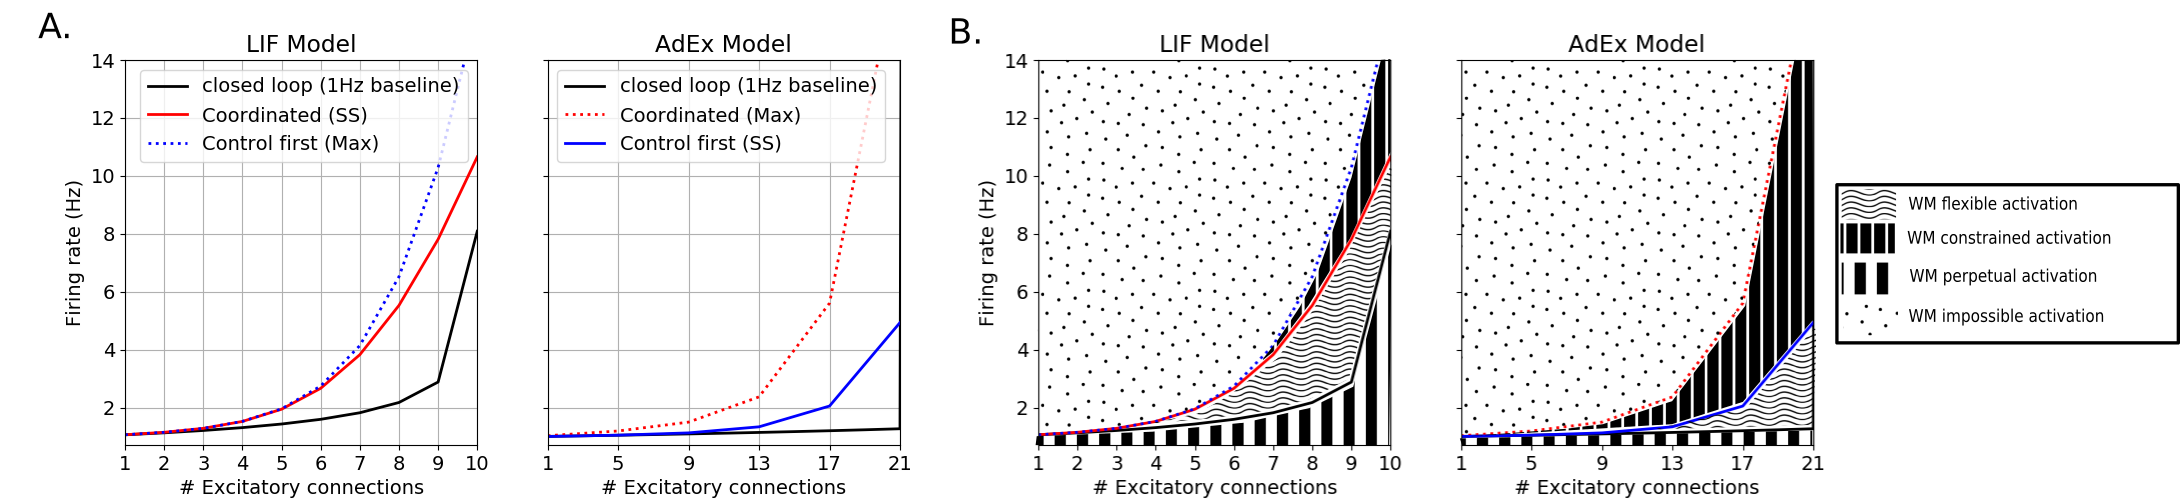
\includegraphics[width=0.70\columnwidth]{figures/experiment_3/experiment_3}

    \caption{Closed loop activity and memory sub-circuit activation regions.
      Plots at the top show an example steady state and max activity rate of the event combination with weaker rate dynamics, in contrast to the steady state rate of the closed loop enhanced activity formed by WM activation.
      Plots at the bottom identify the parameter regions, where the WM steady state rate (SSR) and maximum rate (MR) threshold region is the one that gives most constrained range of circuit parameters to offer the most flexible coordination of input and control events.
      The event rate curves correspond to an input rate of 10Hz and 25Hz for the LIF and AdEx models respectively.}
    \label{197355}

  \end{center}
\end{figure}

\subsubsection{Experiment 4: Inhibition of closed loop enhanced neural
  activity}

{\label{554287}}

For the fourth and last sub-circuit experiment, corresponding to topology D of Figure 4.
We aimed at tuning the amount of inhibitory connections in the circuit such that the neural activity in GKs could inhibit the activity in Gs when there is no intervention of control signals.
In this way we break permanently the closed loop of activity unless a bidirectional control signal or WM activation allows it in the complete circuit dynamics.
To realize this we picked the number of inhibitory connections necessary to inhibit max firing rates for the wide range of number of excitatory connections allowed by the closed loop dynamics.
The maximum firing rate is employed instead of the steady state rate to observe inhibition of the strongest fluctuations.
Based on the curves shown in Figure 8,~we set the number of inhibitory connections to 70 and 250 for LIF and ADEX populations respectively for the following simulations.



\begin{figure}[h!]
  \begin{center}
    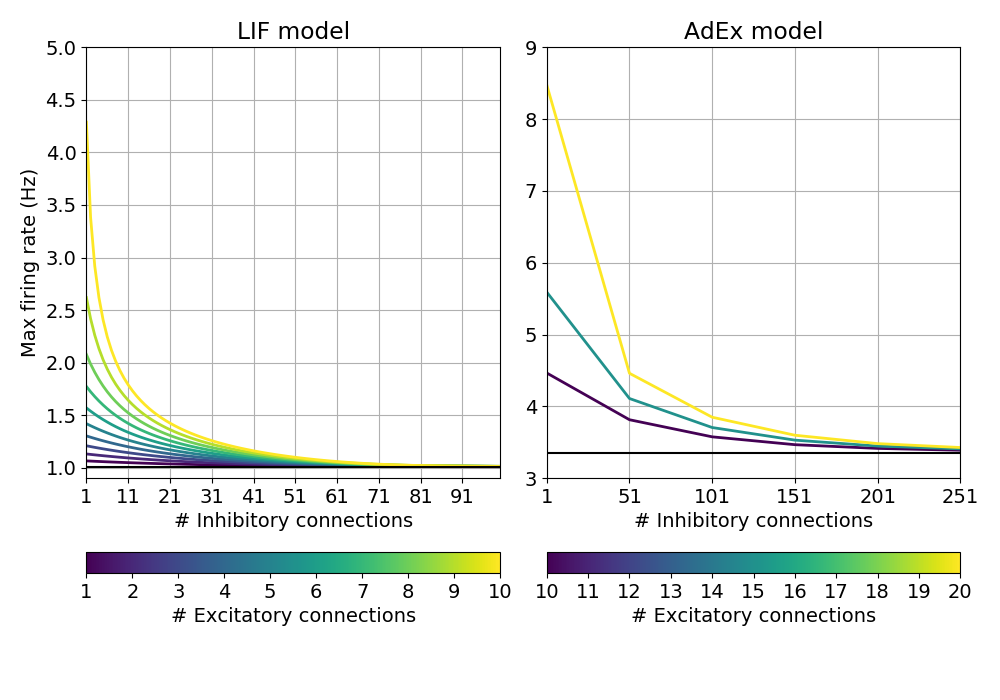
\includegraphics[width=0.70\columnwidth]{figures/experiment_4/experiment_4}
    \caption{Inhibition of closed loop neural activity.
      Each curve represents how the maximum enhanced
      neural activity of ~a closed loop circuit with a given number of
      excitatory connections is driven back to baseline as we increase
      the number of inhibitory connections.
Considering a baseline
      rate approximating a 1 Hz steady state in both Models.
The
      maximum firing rate is employed instead of the steady state rate
      to observe inhibition of the strongest fluctuations.
}
    \label{970310}
  \end{center}
\end{figure}

\subsection{Complete compartment circuit simulations}

{\label{444332}}

After selecting a valid set of parameters from the observations of the sub-circuit experiments we explored the behavior of the complete compartment circuit simulation.
The dynamics of the compartment circuit can be summarized by a combination of the input events that drive activity in MAs and the control events that inhibit GKs such that activity can flow from MAs to Gs and SAs.
In Table 1 we present a summary of the parameters for LIF and AdEx simulations and in Figure 9 we present the temporal dynamics of the compartment circuit under different combination of events.

\begin{table}[h!]
  \centering \normalsize
  \begin{tabular}{ccc}
    Parameter & LIF & AdEx \\
    baseline connections & 115 & 1646 \\
    excitatory connections & 8 & 20 \\
    inhibitory connections & 70 & 250 \\
    Baseline rate (Hz) & 10 & 20 \\
    WM/Ctl rate (Hz) & 10 & 20 \\
  \end{tabular}
  \caption{Complete simulation parameters}
  \label{917316}
\end{table}

First we observed the dynamics of the circuit when no event take place, leading to baseline activity.
In this state all biological populations are just receiving an input baseline rate of 1 Hz from the artificial baseline neural population.
Nonetheless instead of having an output rate approximating 1 Hz as they would have in isolation, the different nodes reflect with their firing rate the architecture of the circuit.
Gs show a low rate of activation due to GKs inhibition, while GKs how the highest rate driven by MA and baseline activity.
MAs show an activation close to the approximated 1Hz baseline as well as SAs that have been isolated in the circuit thanks to GKs inhibition.
SAs have a slightly higher steady state rate than MAs since they are the center recipient of neural activity of the circuit and at least some neural activation manages to leak the Gs.
The baseline activity of the different neural models can be seen in part A of figure 9.

Then in part B of Figure 9 we portray the partial activity of the circuit.
This means that only one MA receives a fix input rate and a Ctl event takes place opening activity flow from both MAs to SAs.~We can observe that, as expected, the increased activity of the stimulated MA causes strong inhibitory activity in the GK that compensate the flow of neural activity from MA to G to avoid activation of the corresponding SA.
Moreover it can be seen in Figure 9 that in the case that Ctl activation takes place when only one MA is active, the circuit effectively do not activate the binding WM and will simply return to an appropriate steady state once Ctl stops.

Finally in part C of Figure 9 we can appreciate that in case both MAs are active and a Ctl event takes place, then the binding will take place by activation of WM.~During the process of binding the reverberating activity of WM that inhibits the GKs connecting SAs creates a sudden burst of activity leading to a pronounced spike as SAs become part of a self excitatory closed loop, also elevating the activity of Gs and GKs between them.
This burst of activity quickly drops back to a steady state that leaves the inner circuit in a higher level of activity with respect to its original resting state, facilitating communication between MAs.
A similar behavior during sentence parsing was observed in previous simulations of the NBA\cite{Frank_2014}.

Although the general qualitative behavior of the compartment circuit architecture is similar for LIF and AdEx populations, there are three important quantitative differences present but not easy to appreciate in Figure 9.
The first is that LIF population dynamics take longer to transmit rates of activity since its transient oscillations are more modest in proportion to the input rate.
In these simulations, with the same timing of events, WM became active 86 ms after all input and control events take place in the LIF simulation, while in the AdEx simulation this only took 42ms.
The second is that the new enhanced activity regime produced by WM activation is very sensitive to the adaptation effect present in the AdEx model.
Not only the parameters of the neural model itself but also synaptic efficacy could completely eliminate the higher sustained activity while keeping a high spike of activity on the moment that binding takes place.
The third is that the AdEx simulation is sensitive also to small variations in the timing of events due to the increasing influence of adaptation as populations reach the steady state, while LIF model dynamics are only affected by the input rate of the events.

\begin{figure}[h!]
  \begin{center}
    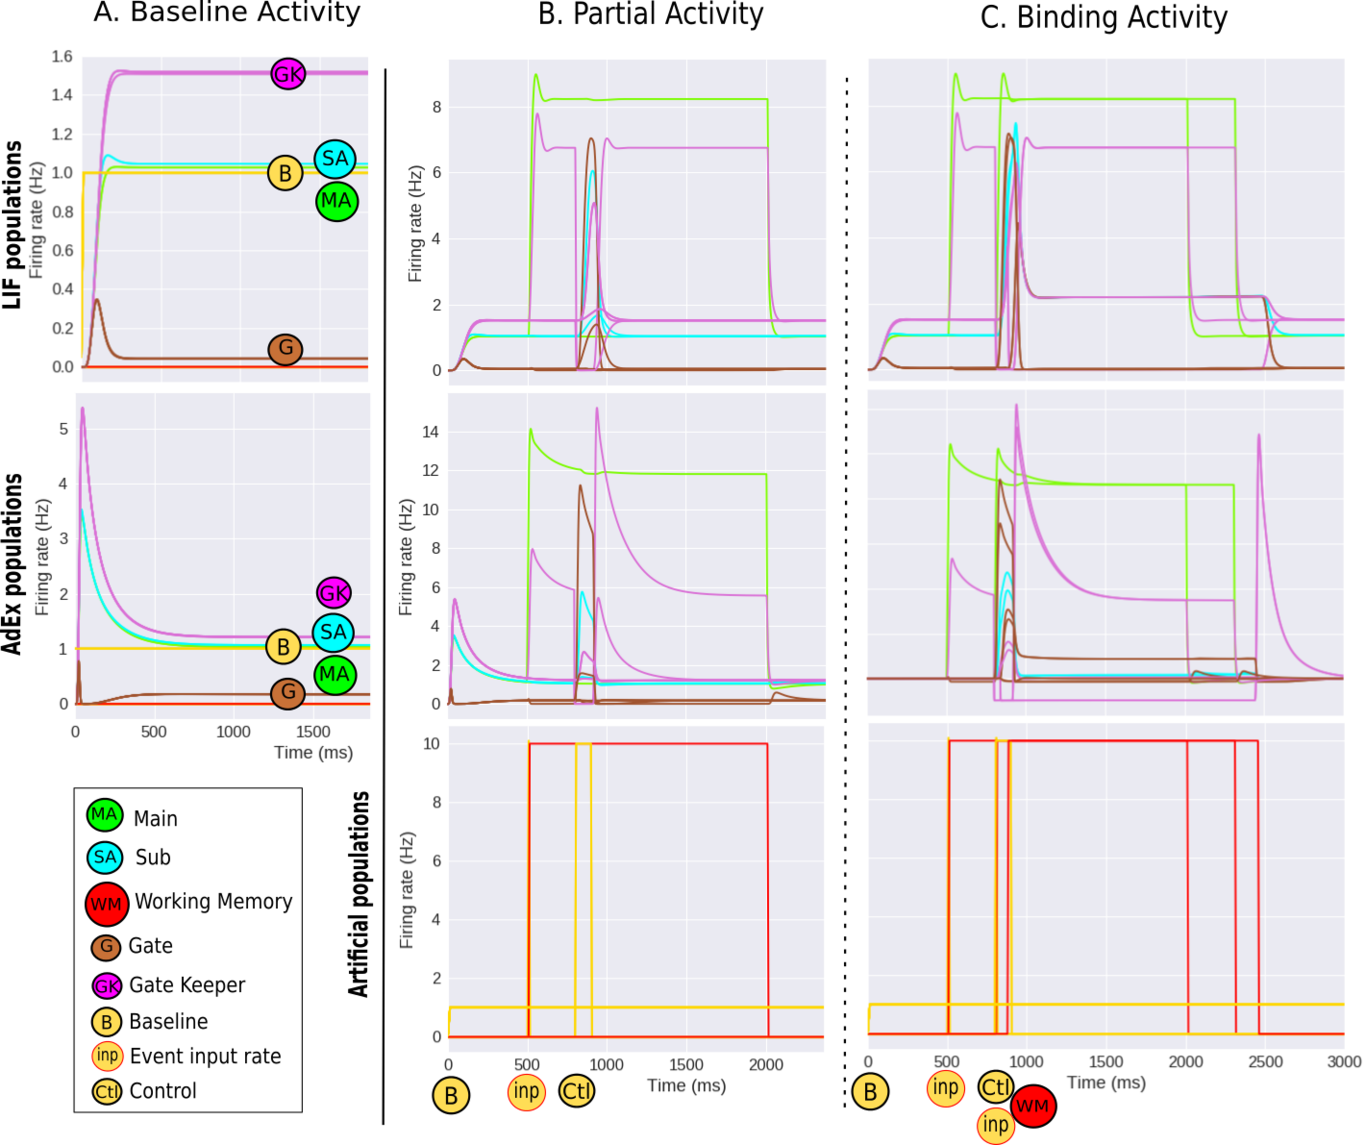
\includegraphics[width=0.70\columnwidth]{figures/compartment_circuit_dynamics/compartment_circuit_dynamics}
    \caption{Profiles of neural activity.
      \textbf{A.} Neural activation driven only by baseline input. \textbf{B.} Neural activation of the circuit when only one MA is activated by a word event or WM at 500ms.
      Portrays the neural activity related to an erroneous control signal at 800ms.
      It is possible to see that the steady state of neural activity is resilient to a slip of control, going to the appropriate levels of neural activity once the control activity is over.
      \textbf{C.} Neural activity of the Compartment Circuit for a successful binding.
      The second MA gets activated at 800ms alongside the controls.
      Since both MAs are active, the SAs manage to activate WM to instantiate the binding of the MAs.
      Two interesting dynamics arise from the binding.
      The first is that a spike of activity in SAs, GKs and Gs takes place due to the sudden inhibitory activity of WM on the GKs.
      The second is that the memory circuit internally raises its baseline activity.%
    }

      \label{activity_profiles}
  \end{center}
\end{figure}

Once we have the neural dynamic of the compartment circuit, we can extract key segments of transient activity and approximate the NBA binding activity of complete phrases.
For this approximation we can consider parallely the necessary compartment circuits to build an assumed underlying tree data structure given by a grammar theory.
We would also need a specification of the timing of parsing operations and the desired duration of WM activity.
The order of the parsing operations can be taken from a bottom-up or more generalized left-corner parsing scheme.
Then the more precise timing of the parsing operations can be assumed to depend on word presentation times for word bindings and minimal operational constraints.
Furthermore, we can think of the WM of word bindings as the MAs of phrasal nodes and so on, which would then give us the time at which a superior phrasal nodes input is available.

One can see in the example of Figure 10 how the hypothesized tree structure of a sentence and the timing of the activation of tree nodes is transformed into the neural activity of a blackboard.
First we substract the baseline activity profile from the binding activity profile of the segments of neural dynamics used for the simulation.
This is motivated by our interest in making comparisons with neuroimaging data.
Then we simply add up the aligned time series of the different compartment circuits by neural population category or some other desired criteria.
In the example, summaries of the activity of different neural populations are shown as well as total activity of the blackboard circuit assuming equal contribution from the different populations.
Certainly the way we should aggregate time series to compare them quantitatively with neuroimaging data would depend on the spatial and temporal resolution available and the assumptions made about the spatial distribution of the blackboard architecture in the cortex.
in the case of WM activation it is reasonable to assume a duration at least long enough to allow all bindings in the tree to take place at the rate that words are presented to the blackboard.
In this example words are presented every 600 ms, so for illustrative purposes we assume WM is active 2300ms to be able to bind the first word to an awaited phrase node activated after presentation of the fourth word.
If WM was active for say less than 1900ms then activation of the first word MA would cease before the accompanying phrasal node MA comes into play.

\begin{figure}[h!]
  \begin{center}
    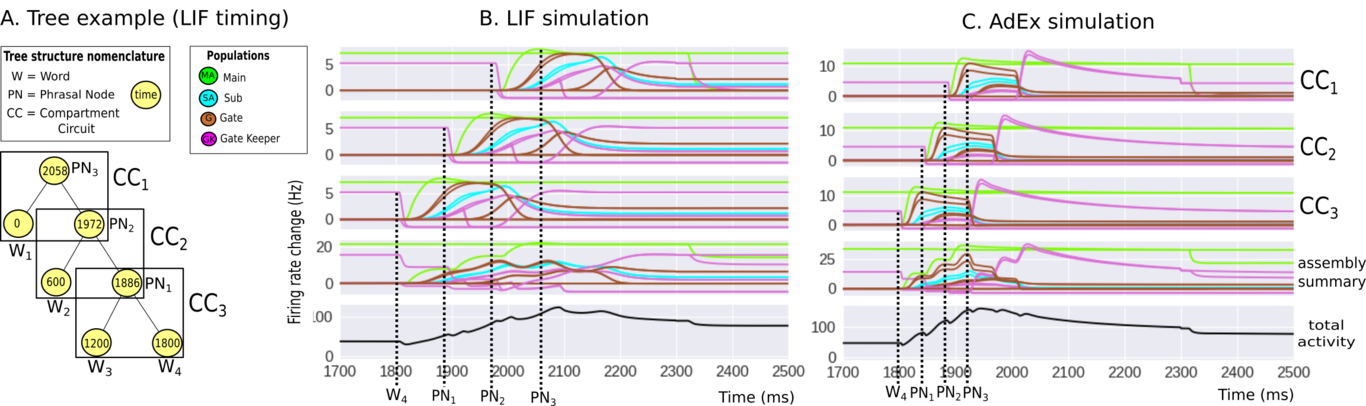
\includegraphics[width=1.00\columnwidth]{figures/compartments_tree_example/compartments_tree_example}
    \caption{Sentence processing example.
      A. Tree structure hypothesized for a given 4 words phrase.
      It is shown how compartment circuits correspond to sections of the tree structure and how the nodes corresponding to grammatical categories of words processed or phrase nodes are instantiated in time under a bottom-up parsing approach.
      B. Blackboard time series that correspond to the simulated processing of the considered tree structure and time of activation of the nodes.
      The separate activity of the LIF populations of each compartment circuit are shown separately, followed by their summary and total activity.
      C. Same as~B but for AdEx populations. {\label{679921}}%
    }
  \end{center}
\end{figure}


\subsection{Qualitative reproduction of neuroimaging patterns}

{\label{444332747980}}

We can apply the complete phrase neural time series approximation to a variety of stimuli from experimental designs behind neuroimaging results in the literature.
First we considered the simple case of increasing size right branching trees that relate to a recent analysis of intracortical (ECoG) recordings of a phrase reading task\cite{Nelson_2017}.
In this experimental design subjects had to keep a phrase in memory to later compare it with a shorter probe phrase.
We make a qualitative comparison with caution, given that high gamma power has been shown to be correlated to the firing rate time series of spiking neurons from in-vivo recordings\cite{Ray_2011}.~In our simulation, shown in Figure 11.A, we can appreciate four main temporal segments of neural activity.
An initial increase of activity dependent on word presentation that reflects MA populations, a sudden rise and drop of activity during WM activation, a decrease of activity paced by the duration of input activity driving MA populations and a final drop of activity when WM delay activity stops and the inner closed loop of populations in the memory sub-circuit go back to its initial baseline state.
We also show, in Figure 11.B and 11.C., modified plots, extracted from Nelson et al., reflecting the mean high gamma power time series of the ECoG recordings.

As can be seen in Figure 11.B, there is an increase in baseline activity when comparing the beginning and end of phrase processing that can be interpreted as WM related activity based on the task.
This memory effect is reproduced in the NBA simulation by the enhanced activity of the closed loop in the memory sub-circuit.
It is represented by the difference between the start of the simulation and the end of the MA inactivation temporal segment, denoted in Figure 11 by black bars.
It could further be tuned to fit quantitatively the data by manipulating the number of excitatory connections, such that their decrease would reduce the baseline difference.
The irregularities of the magnitude of the baseline effect with respect to phrase length in the high gamma power is difficult to interpret, since it could suggest that the accumulation of activity with more recruiting nodes is subtler than what we can reproduce with the NBA circuit, in which there is a clear correspondence with the number of hypothesized compartment circuits of the parsed tree structure.
Moreover, when comparing simulations, we appreciate that the AdEx model could better reflect a more modest proportional increase of baseline thanks to adaptation.~

Another observation of the experiment is a proportionally important ~increase in activity during word processing.
The peak magnitude and onset of this increase seems to reflect the length of the phrase.
This effect can be captured by the simulation with a simple interpretation of the accumulation of MA activity waiting to participate in bindings, assuming a bottom-up parsing scheme.
Nonetheless what was unexpected is the spike of activity followed by a pronounced drop suggested naturally by the NBA simulation, which is also emphasized by Nelson et al. in Figure 11.C.
This seems to be the case for both intermediate and final bindings, with a drop magnitude dependent on the number of open nodes in the assumed phrase grammar tree structure of the phrases.
The number of open nodes reflect accumulation of pending bindings under a bottom-up parsing scheme in right branching sub-trees.
The increasing drop magnitude is captured in the simulation by the quick succession of pending bindings in a tree structure.
In the case of the LIF simulation, there is flexibility to extend the activity peak with the duration of control events and to increase the total drop magnitude by manipulating the input rates and excitatory connections.
On the other hand the AdEx model loses this flexibility due to adaptation but better emphasizes the contrast between the activity peak and sudden drop because of the pronounced initial activity burst of its population dynamics.

There~is an issue with the interpretation of activity drops due to binding operations.
As can be seen in Figure 11.B, for the assumed right branching phrase ``ten sad students of Bill Gates'', there is a sentence middle drop that do not correspond to the prediction of a completely bottom up parsing scheme.
To accommodate this behavior into the NBA, without changing our grammar and parsing assumptions, we would need to incorporate a limited capacity to sustain MA activity that has to be renovated or a greedy binding mechanism that leads to premature binding mistakes.
In the case of the sentence end, the final activity drop has a steeper slope than the activity raise during sentence processing, suggesting to incorporate a mechanism that releases MA activity after binding takes place, which is unaccounted for in the simulation.
Finally in the analysis of Nelson et al. there is no depiction of WM inactivation, likely due to the experimental design.
Interestingly, the AdEx simulation distinguishes itself from the LIF simulation, during WM inactivation, by predicting a final burst of activity due to the inhibition release of the GKs in the memory circuit.
Nonetheless this would be a difficult to appreciate marker in the oscillatory signal of intracortical recordings.

\begin{figure}[h!]
  \begin{center}
    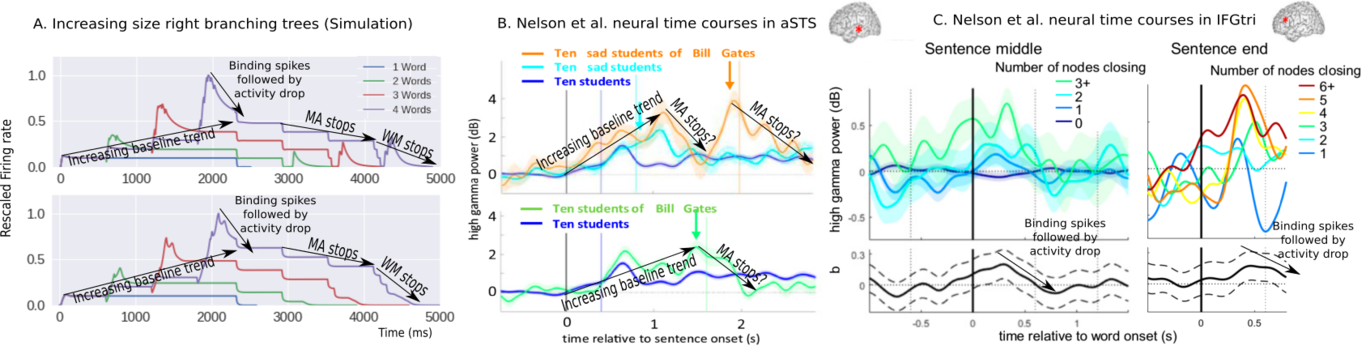
\includegraphics[width=1.00\columnwidth]{figures/ecog_comparison2/ecog_comparison2}
    \caption{{Simulation comparison with intracortical (EcoG)
        recordings {\label{286166}}%
      }}
  \end{center}
\end{figure}

We also considered the case of a more complex experimental design employed to show constituency effects with Bold-fMRI\cite{Pallier_2011}, also based on right branching trees.
In this experiment each stimuli presented to a subject in a trial consisted of a list of phrases with the same number of words (constituents), such that in total 12 words would be presented.
The conditions were one list of 12 unconnected words (c01), 6 phrases of 2 words (c02), 4 phrases of 3 words (c03), 3 phrases of 4 words (c04), 2 phrases of 6 words (c06) and 1 phrase of 12 words (c12).
This stimuli was simulated by repeating and adding the time series of~each of the right branching trees in a condition.
In figure 12 we contrast the NBA neural activity time series predicted by the LIF and AdEx simulations for each condition with the simple Boxcar event model used in experiments to estimate the amplitude of the hemodynamic responses.
We applied with a convolution operation, to each time series, the Hemodynamic Response Function (HRF) proposed by Glover\cite{Glover_1999}, taken from the python open source package Nistats (\textbf{MISSING REFERENCE)}.
This is a very naive approximation taken for illustrative purposes, that has to be interpreted with caution since the relationship between neural activity, cerebral blood flow and blood oxygenation is not linear\cite{Friston_2000,Buxton_2004} and better represented by the balloon model than the gamma function considered here\cite{Waldorp_2009}.

In Figure 12 we mark the HRF peak and its onset with black lines on the HRF convolved time series.
It can be appreciated that the neural time series would predict in all cases a peak onset displaced many seconds with respect to the traditional boxcar event that only represents the duration of the stimuli.
Looking at the time series this would be expected, since the HRF peak onset depends on the center of mass of the accumulated response that continues several seconds after stimuli presentation.
Nonetheless a precise onset estimation depends on the MA and WM inactivation periods that have been arbitrarily set in the simulation to a constant, which leads to a superlinear increase of onset based on number of constituents.
This is unlikely from our previous observations in ECoG recordings, that suggest a much faster decrease of activity after stimuli presentation.
Still this prediction gives a cautionary tale on the extent to which lack of neural modelling can lead to a non trivial misspecification of the events introduced in the GLM model to analyze Bold-fMRI experiments.
Thinking the other way around, the peak onset link to the MA and WM inactivation periods suggest that we could also use Bold-fMRI to fit the parameters of an inactivation mechanism in the NBA.
To realize this, such mechanism would need to be proposed and a more realistic mapping from neural activity to blood oxygenation would need to be implemented.
As a last remark related to HRF peak onset, one can appreciate that the LIF neural model introduces an additional onset delay with respect to the AdEx neural model, due to its slower activation of bindings.

\begin{figure}[h!]
  \begin{center}
    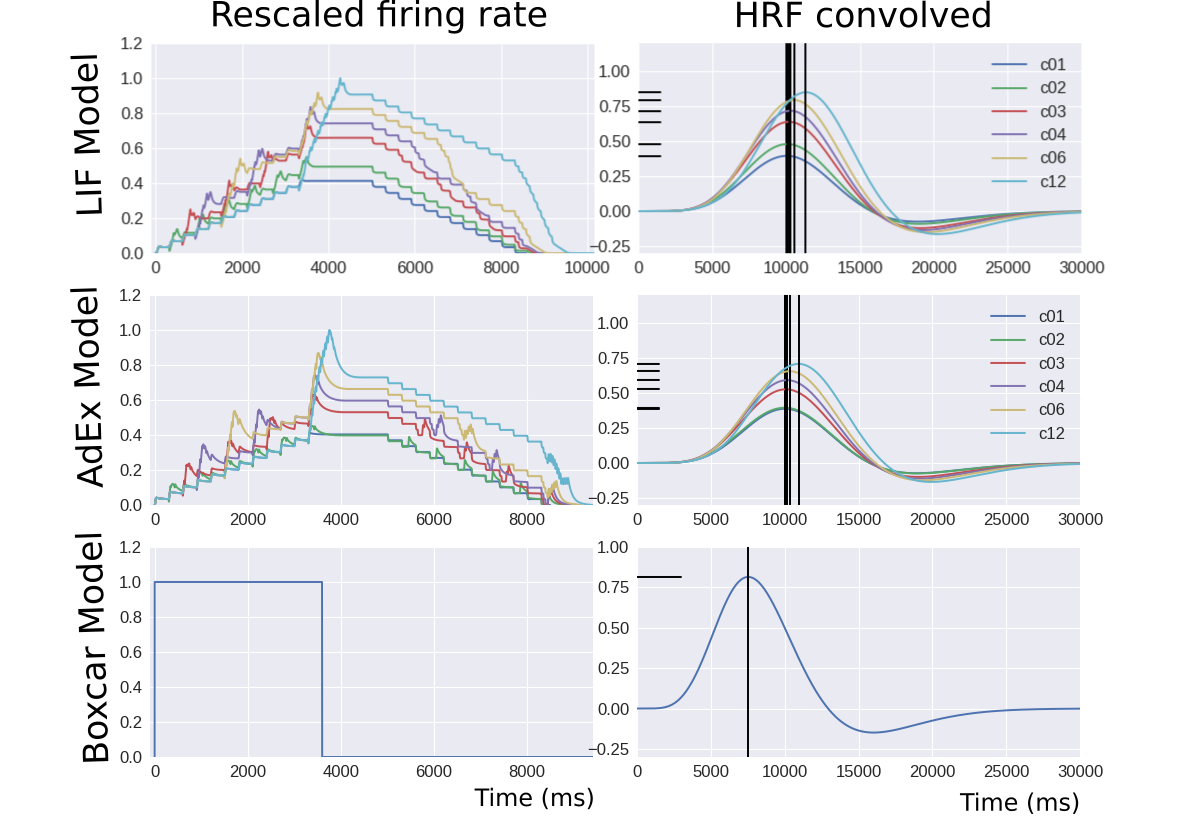
\includegraphics[width=1.00\columnwidth]{figures/pnas_comparison01/pnas_comparison01}
    \caption{{Simulation hemodynamics interpretation {\label{473368}}%
      }}
  \end{center}
\end{figure}

On the other hand, both AdEx and LIF simulations predict a similar pattern on the increase of the amplitude of the HRF peak for conditions with increasing constituent size.
Since the peak depends mostly on the number of nodes of the assumed tree structures, it is more interesting to compare it qualitatively with the experiment.
Our simulations reproduce the sub-linear response that surprised initially the authors, who were testing a linear hypothesis.
In addition to normal phrases, Pallier et al. designed a jabberwocky stimuli in which function words are preserved and other words are replaced by morphological similar but undefined words.
While there are constituent responses in the language areas TP, aSTS, pSTS, TPJ, IForb and IFtri, only the regions pSTS, IFGorb and IFGtri portray a similar response pattern even when minimizing the semantic content of phrases with jabberwocky.
Since our simulation puts aside semantic considerations, this type of experimental manipulation is a better reflection of the activity linked to the compartment circuit of the NBA, in contrast to the aSTS time series previously analyzed on the ECoG dataset.

We portray in Figure 13 the simulations predicted pattern alongside the ones revealed in pSTS, IFGorb and IFGtri language regions for the jabberwocky stimuli.~The LIF and ADEX predictions are very similar, except for the word list condition.
Notice that the contrast of the amplitude of word lists with the other conditions can give insights into the relative proportion between MA and WM activity.
As we saw in the ECoG time series, MA seems to have a more important participation in the total neural activity than we initially modeled.
This could explain the~flatter slope of the experimental results.
To reproduce it with our simulations, keeping their qualitative behavior intact, we could select a parameter regime with less excitatory connections and higher input rate.
Note that in the case of the AdEx model, due to the shape of the adaptive response, it would be possible to reproduce the sublinear peak amplitude effect while minimizing a peak onset difference.
To achieve this we could make all responses approximate the same center of mass by mixing the high initial increase of firing rate, that depend mostly on the input rate, with a very low steady state rate.
Nonetheless, to make a quantitative fit to the hemodynamic amplitudes we should use a more realistic hemodynamic model and be cautious about the possible model misspecifications introduced by the simultaneous consideration of the HRF peak onsets.

\begin{figure}[h!]
  \begin{center}
    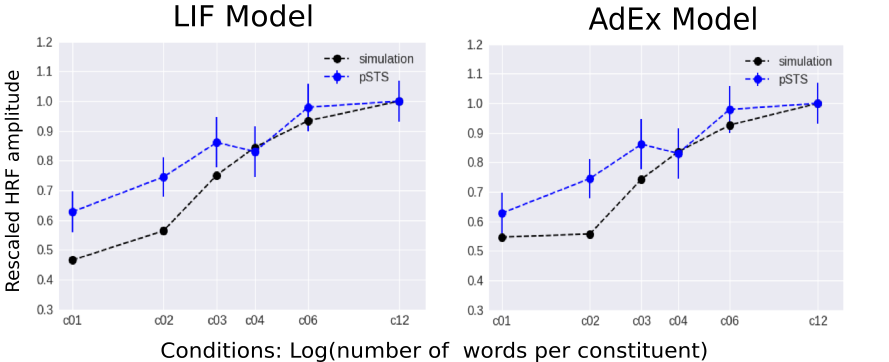
\includegraphics[width=1.00\columnwidth]{figures/pnas_comparison-02/pnas_comparison-02}
    \caption{{Simulation comparison with Bold-fMRI experiment
        {\label{395077}}%
      }}
  \end{center}
\end{figure}

\section{Discussion}

{\label{160055}}

An important insight from this work is the sensitivity of the neural activity interpretation to the underlying neural model selected.
Even in the case of hemodynamic responses that average out circuit details, we find trade-offs between the LIF and AdEx models.
For example that an AdEx model would offer more flexibility in our circuit to manipulate HRF peak amplitudes while minimizing their onsets.
To our knowledge this is the first work to explore more complex models like AdEx alongside LIF for variable binding and language function related circuits.
There were also many predictions of the NBA independent of the model selected, like the fact that we need a high number of inhibitory connections and so of inhibitory activity to avoid uncontrolled regimes of self excitatory activity dependent on the connectivity of the circuit.

A more subtle exploration that was considered out of the scope of the work would be to appropriately consider the cell parameters in the models based on electrophysiological recordings from specific brain regions, in contrast to the Omurtag~\cite{omurtag2000simulation}~Brette et al. parameters~\cite{Brette_2005}.
There are indeed different adaptation constants along the cortex and we have compared the simulation constantly with specific language related brain regions like aSTS, pSTS, IFGtri and IFGorb.

In the case of the complete circuit assumptions, some of them were still overly simplistic.
We approximate baseline dynamics with a simple low constant input rate instead of also considering the natural oscillatory activity of the cortex, more appropriate homeostatic mechanisms in cortical circuits\cite{turrigiano2011too} and balanced networks\cite{Wolf_2014}.
Setting up the synaptic distribution of the network have important implications in terms of energy consumption, while allowing random connectivity could importantly constrain control of closed loop connections.
This last consideration is interesting in itself as a research question and could have an impact in the study of the temporal bottlenecks observed in language processing\cite{Vagharchakian_2012}.
Introducing modular cytoarchitectonic considerations on the populations that conform the circuit would allow a better spatial interpretation of the circuit activity in a cortex patch and might be anyway necessary to accurately translate firing rates into Local Field Potentials\cite{Mazzoni_2015,Hagen_2015}, hemodynamics~\cite{Buxton_2004} and other promising measurement techniques.

Moreover the nature of WM delay activity was left out of the current work due to its flexible and still debated implementation\cite{de_Kamps_2005}, but studying it could reveal important neurobiological limitations on the way we asses the proportion of MA and WM activity and the spatio-temporal memory limitations of the circuit.
A final missing consideration that has been partially tackled in previous work\cite{van_der_Velde_2011} is how such a circuit architecture can be formed during learning and brain development.
We obviously do not expect the hardwired architecture modeled here to represent the biological reality but to facilitate an approximation to its behavior.
Demonstrating how mechanisms approximated by the architecture can actually be learned with biological realistic Hebbian or STDP rules alongside random connectivity constraints, during development, is an important avenue of future research.

The simulation results show how both the steady state and transient dynamics of the circuit affect our interpretation of the neuroimaging evidence for language processing.
In contrast to previous simulations\cite{van_der_Velde_2011,van_der_Velde_2010,Frank_2014,van_Dijk_2015}, employing population density techniques implemented in the MIIND software\cite{de_Kamps_2008} allowed us to approximate well transient temporal dynamics.
Thanks to this, we could show an important difference in the shape of the AdEx and LIF responses, how before arriving to a steady state AdEx responds differently to additional input due to adaptation and how the coordination of input and control events is importantly influenced by the model and its parameters.
This last point is crucial for language processing, since ideally~we would want input and control events to be as independent as possible to diminish operational complexity and to be able to operate under a wide range of parameters allowing for random variation.
Reflecting on the coordinating complications introduced by adaptation we would expect lower adaptation in language related brain regions that seem to be involved in binding operations like pSTS, IFGTri and IFGorb, an increase in the operational complexity of the circuits and/or a reduction in the operational parameter ranges alongside additional sensitivity to noise.
A final remark related to event coordination problems in AdEx would be its sensitivity to the synaptic efficacy parameter of the circuit that was not explored in detail.
Contrary to the LIF model, AdEx requires clear limitations in the populations connectivity to implement arbitrary or complex timing operations.

An important aspect of this work, that could be overlooked, is the flexibility of the simulation to represent the neural activity of many grammar theories and parsing schemes.
We can without circuit modification implement any concept represented as a binary tree.
This corresponds well for example to the phrase grammar of the minimalist program of Chomsky\cite{Chomsky_2014}~and to grammatical relations in dependency grammars\cite{nivre2005dependency}.
Nonetheless in the case of dependency grammars we would not need to extend the memory of MA less than in a phrase grammar that requires to wait for the instantiation of phrase nodes in deep hierarchical trees.
Also the AdEx model would favor shallower tree representations, because it is sensitive to complex event coordination.

Also so far we have implicitly considered activation of phrase nodes only as a result of word binding, which would be representative of a bottom-up parsing approach.
This allowed us to simply take the binding WM activity of one compartment circuit as the MA of another compartment circuit.
Nonetheless we did not introduce additional delays in control, since we did not model the portion of the NBA responsible for control.
Naturally there are many additional parsing mechanisms that we could assume, represented by the order of input and control events, that would introduce predictive control activity.
This would be the case if we extend our analysis to the~generalized left corner parsing proposed by Hale\cite{hale2014automaton}.
We could interpret this additional predictive control signals as control anticipation or as direct activation of memory circuits that have to be deactivated later by an error signal.
Exploring the neural activity implications of both these mechanisms alongside the target tree structures given by alternative grammar theories is an important target of future research.
This could be done for example by using the simulation as an experiment design tool that provides the set of phrases that maximize the spatio-temporal differences in neural responses across conditions defined under the different grammar theories and parsing schemes.

Finally, even though there are still many limitations in these simulations, we would like to emphasize the quick progress in the development of biologically plausible models of cognition.
With an additional effort it would be possible to fit parameters of the circuit and phrase processing directly to neuroimaging measurements.
Also diverse new computational methods like population density techniques have made it feasible to approximate at a circuit scale point neural models as complex as the adaptive exponential.
There are as well successful recent efforts in modeling, with cytoarchitectonic details, complex signals like Local Field Potentials~\cite{Mazzoni_2015,Hagen_2015} and hemodynamics with the balloon model~\cite{Buxton_2004}.
These could be already adapted to our circuit simulations to better incorporate neuroimaging evidence simultaneously from multiple techniques and experimental designs.
Moreover the circuit itself can become a tool for hypothesis exploration and experimental design on the different neuroimaging techniques.
In conclusion we hope~to have shown that we are close to producing biologically realistic mechanistic neural models of cognitive function, that could provide new ways of testing cognitive hypothesis on varied neuroimaging techniques, to further~inspire more work in this direction.


///////////////////// POSSIBLE ADDITIONS TO DISCUSSION (IGNORE)

ADD TO DISCUSSION BUT MAYBE ALSO TO NEUROIMAGING RESULTS A REFLECTION ON THE NUMBER OF CIRCUITS RECRUITED FOR BINDING AS AN EXPLANATION FOR THE SUB LINEAR EFFECT, SO OUR MODEL WOULD PROPOSE A NEW PREDICTION WITH DIFFERENT COMBINATIONS OF PHRASES COMPLETELY BASED ON THE NUMBER OF COMPARMENT CIRCUITS IMPLIED BY THE GRAMMAR. THEN I CAN DISCUSS THE PROBLEM IF WE CHANGE THE GRAMMAR, WHAT WOULD A DEPEDENCY GRAMMAR PREDICT AS NUMBER OF COMPARTMENT CIRCUITS?


Comment on the possible extension of the model to other linguistic hypothesis like dependency grammars that consider the words directly as nodes? instead of having phrasal nodes?


The compartment circuit abstraction is enough to achieve our current simulation goals\noteCP{Would be nice to list them early in the paper.}, since the same mechanism is used in different connection matrices and they might only differ in their memory capacity.
So we can consider the same compartment circuit simulation for all different pairs of grammatical categories, where the circuits would have similar dynamics and only vary in activation time of their neural populations.
Nonetheless we are only able to ignore the activity of complete connection matrices because we are not planning to explore the effect of memory limits under time compressed sentence processing scenarios or memory tasks.
Otherwise important deviations in background neural activity due to depletion of available compartments in the connection matrices and intense inhibitory activity would become a crucial factor in the simulation.
This could be an interesting exploration in future work to try to reproduce the temporal bottleneck effects on neural activity shown by Vagharchakian et al. under conditions of compressed speech and reading\cite{Vagharchakian_2012}.\noteCP{Maybe this should be part of the final discussion rather than here where it may divert attention.}


Maybe clarify that top-down considerations of parsing could be reflected in MAs activated by a prediction mechanism, in Ctl anticipating activation of certain MAs in the blackboard or by parallel instantiation where WMs are later inhibited by error signals.
That we have the flexibility to test arbitrary computational linguistic mechanisms with the NBA but that interpretation requires further considerations that we leave out of the scope of this work.
where bottom up is employed.


Here we implement only the necessary parts of the NBA to model the neural activity related to variable binding, which itself is enough to instantiate the representation of an arbitrary sentence syntactic structure
\noteCP{What you mean here, is it is enough to have a CONS-like operation --- in LISP parlance --- to build any tree, right?}
if we take the grammar theory and parsing scheme as given.
\noteCP{Think about the reader who does not know the distinction between grammar theory and parsing The previous paragraph, with more details, could explain it.
Or get reif of it.
This may actually not be an important distinction for the purpose of this paper}.
This means that we simplify two important aspects of the circuit.
The first is that we will provide the signals of control directly to the compartment circuits.
Previous attempts to train the control mechanism\cite{van_der_Velde_2010} were tailored only to specific grammatical cases and creating a general control mechanism to test the neural activity patterns would require a more varied dataset in grammatical categories
\noteCP{???}
and would comprise computational linguistic efforts out of the scope of this work.
The second is that we do not model the dynamic inhibition of competing blackboard compartment circuits, since this would require an hypothesis about the size of the blackboard, which would be related to memory limitations and the total number of possible grammatical categories to link in binary trees, which again would require out of scope computational linguistic efforts.
\noteCP{More of a psycholinguitics issue than a computational linguistics one, no?}.
Moreover the simplest selection mechanism behind competing blackboard compartment circuits can be hypothesized to be uniformly random on available compartments.
This means that we are only testing the temporal patterns of neural activity linked to a variable binding event in the case of two words association.
\noteCP{But but but, you are also modeling the binding of a word and a phrase, no?}
While in the case of complete sentences we are testing predictions based on the average neural activity time series of a collection of compartment circuits instantiated as demanded by the given grammar theory and parsing scheme.
These time series should allow us to differentiate neural activity from different syntactic tree morphologies and sizes.



\selectlanguage{english}

\bibliography{bibliography/converted_to_latex}

\end{document}

